\chapter{Metodología de la Investigación}
\section{Diseño de la investigación}
En esta sección del documento se explica cuál fue el diseño, el tipo y el enfoque del trabajo de investigación, así como también la población y la muestra. 

\subsection{Tipo de la investigación}
Para determinar el tipo de la investigación, primero fue necesario definir el actual trabajo como Diseño Experimental ya que, según \cite{bk_hernandez2014metodologia} en su libro \citetitle{bk_hernandez2014metodologia}, se pretende establecer el posible efecto de una causa que se manipula. Dentro de esta categoría se clasifica como Diseño Experimental Puro, ya que se manipuló intencionalmente más de una variable independiente (fueron agregadas y/o removidas) con la finalidad de medir el efecto que estas generan en la variable dependiente, el estado final de financiamiento de un proyecto de tecnología en Kickstarter.

\subsection{Enfoque de la investigación}
El presente trabajo tuvo un enfoque cuantitativo ya que, según \cite{bk_hernandez2014metodologia} en su libro \citetitle{bk_hernandez2014metodologia}, este enfoque utiliza la recolección de datos para probar hipótesis con base en la medición numérica y el análisis estadístico, con el fin de establecer pautas de comportamiento y probar teorías. Esto se refleja en los 10 pasos del proceso cuantitativo descritos por el anterior autor y que fueron aplicados en la investigación, desde la concepción de la idea hasta la elaboración del reporte de resultados.

\subsection{Población}
La población fueron todos los proyectos de la web de crowdfunding Kickstarter.

\subsection{Muestra}
La muestra fueron 27,251 proyectos, incluyendo exitosos y fracasados, de la categoría Tecnología, de la web de crowdfunding Kickstarter, entre los periodos 2009 y 2019. Como se mencionó en el Capítulo I, el criterio de la elección de esta categoría se debe a su bajo ratio de éxito de financiamiento en promedio durante los periodos mencionados, los cuales se consideraron hasta el 2019 dado que tomar el año 2020 incurriría en la distorsión del ratio por la coyuntura de la pandemia del Covid-19.

\subsection{Operacionalización de Variables}
En la Tabla \ref{3:table1} se presenta la operacionalización de variables para la investigación.

%\begin{table}[h!]

\begin{longtable}{M{5cm}M{4.5cm}M{5.5cm}}
	\caption[Matriz de operacionalización de variables]{Matriz de operacionalización de variables.}
	\label{3:table1}
	\newcommand{\multirot}[1]{\multirow{2}{*}[-8ex]{\rotcell{\rlap{#1}}}}
	\centering
	\small
	\tabularnewline \specialrule{.1em}{.05em}{.05em}
	VARIABLE & INDICADOR & CÁLCULO/VALORES
	\\%%[5pt]
	\specialrule{.1em}{.05em}{.05em}
	\multirow{2}{5cm}[-2ex]{\centering Estado de financiamiento de un proyecto} & Proyecto exitoso & Monto meta $\leq$ monto contribuido                                                   \\%%[10pt]
	\cline{2-3} & Proyecto fracasado & Monto meta $>$ monto contribuido \\%%[10pt]
	\hline
	\multirow{1}{5cm}[2ex]{\centering Aprendizaje Profundo Multimodal} & Modelo de Aprendizaje Profundo & \setlist{nolistsep}
	\begin{itemize}[label={--},noitemsep,leftmargin=*]
		\item Perceptrón Multicapa
		\item Red Neuronal Convolucional
		\item LSTM Bidireccional
	\end{itemize} \\
	\hline
	\multirow{2}{5cm}[-6ex]{\centering Método de pre-procesamiento} & Normalización de variable cuantitativa & Variable cuantitativa escalada en rango [0; 1] \\
	\cline{2-3}
	 & Procesamiento de Lenguaje Natural &
	 \setlist{nolistsep}
	 \begin{itemize}[label={--},noitemsep,leftmargin=*]
	 	\item Diccionario de palabras.
	 	\item Incrustaciones de palabras.
	 \end{itemize} \\
	\hline
	\multirow{5}{5cm}{\centering Efectividad del modelo} & Exactitud & $\frac{V.P.+V.N.}{V.P.+V.N.+F.P.+F.N.}$ \\%%[10pt]
	\cline{2-3} 
	& Precisión & $\frac{V.P.}{V.P.+F.P.}$ \\%%[10pt]
	\cline{2-3} 
	& Área bajo la curva ROC & $P( score(x^{+}) > score(x^{-}) )$ \\%%[10pt]
	\cline{2-3} 
	& Sensibilidad & $\frac{V.P.}{V.P.+F.N.}$ \\%%[10pt]
	\cline{2-3} 
	& Puntaje F1 & $\frac{2*Precisi\acute{o}n*Sensibilidad}{Precisi\acute{o}n+Sensibilidad}$ \\%%[10pt]
	\specialrule{.1em}{.05em}{.05em}
\end{longtable}
%\par	%%Salto de linea
%\bigskip
\begin{flushleft}	%%Alinear a la izquierda sin justificar
	\small Fuente: Elaboración propia.
\end{flushleft}
%\end{table}

El trabajo busca resolver el problema de clasificación del estado final de financiamiento de un proyecto implementando un modelo de Aprendizaje Profundo Multimodal.

Como se explica en la subsección 2.3.3, un proyecto de Kickstarter presenta 5 categorías de acuerdo al logro del objetivo de su meta. Dado que se busca predecir si llegará a ser financiado o no, el estudio se delimita a exitoso o fracasado. Para determinar este valor, y según la política “Todo o Nada” de la plataforma explicado en la subsección 2.3.2, un proyecto es determinado como exitoso cuando el monto contribuido al culminar el tiempo de vida de su campaña logra ser mayor o igual a su meta estimada. De lo contrario, es un proyecto fracasado.

El modelo propuesto, alimentado de 3 modalidades independientes presentes en cada campaña de Kickstarter, comprende el ensamblaje de 3 modelos de Aprendizaje Profundo: un modelo Perceptrón Multicapa (MLP), una Red Neuronal Convolucional (CNN) y un modelo LSTM Bidireccional. Para estos 2 últimos, se trabajaron sus datos de entrada con técnicas de Procesamiento de Lenguaje Natural que incluye desde el pre-procesamiento de los textos hasta su conversión en vectores que finalmente fueron entrenados en sus respectivos modelos.

Por último, para poder evaluar la efectividad que este registrará al ser entrenado, su desempeño será evaluado a través de métricas de clasificación de Minería de Datos. Para la investigación, las 5 métricas utilizadas fueron la exactitud, la precisión, el área bajo la curva ROC, la sensibilidad y el puntaje F1, las cuales se describen en la Sección 3.3.2.

\section{Técnicas de recolección de datos}
Los conjuntos de datos recolectados para la investigación se componen de variables cuantitativas (características del proyecto como la meta de financiamiento, montos prometidos, duración de la campaña y otros indicadores financieros) y cualitativas (descripción y comentarios del proyecto). Para obtener los 3 principales datasets, se siguió el flujo de la Figura \ref{3:fig1}. La base de datos de la metainformación fue construída luego de descargar un histórico público de 10 años de la página web “Web Robots” y posteriormente pre-procesarla. Por el lado de la descripción y comentarios de los patrocinadores, se usaron técnicas y herramientas de \textit{web scraping} a partir de los URLs de cada proyecto disponibles en la Metainformación.

\begin{figure}[h]
	\begin{center}
		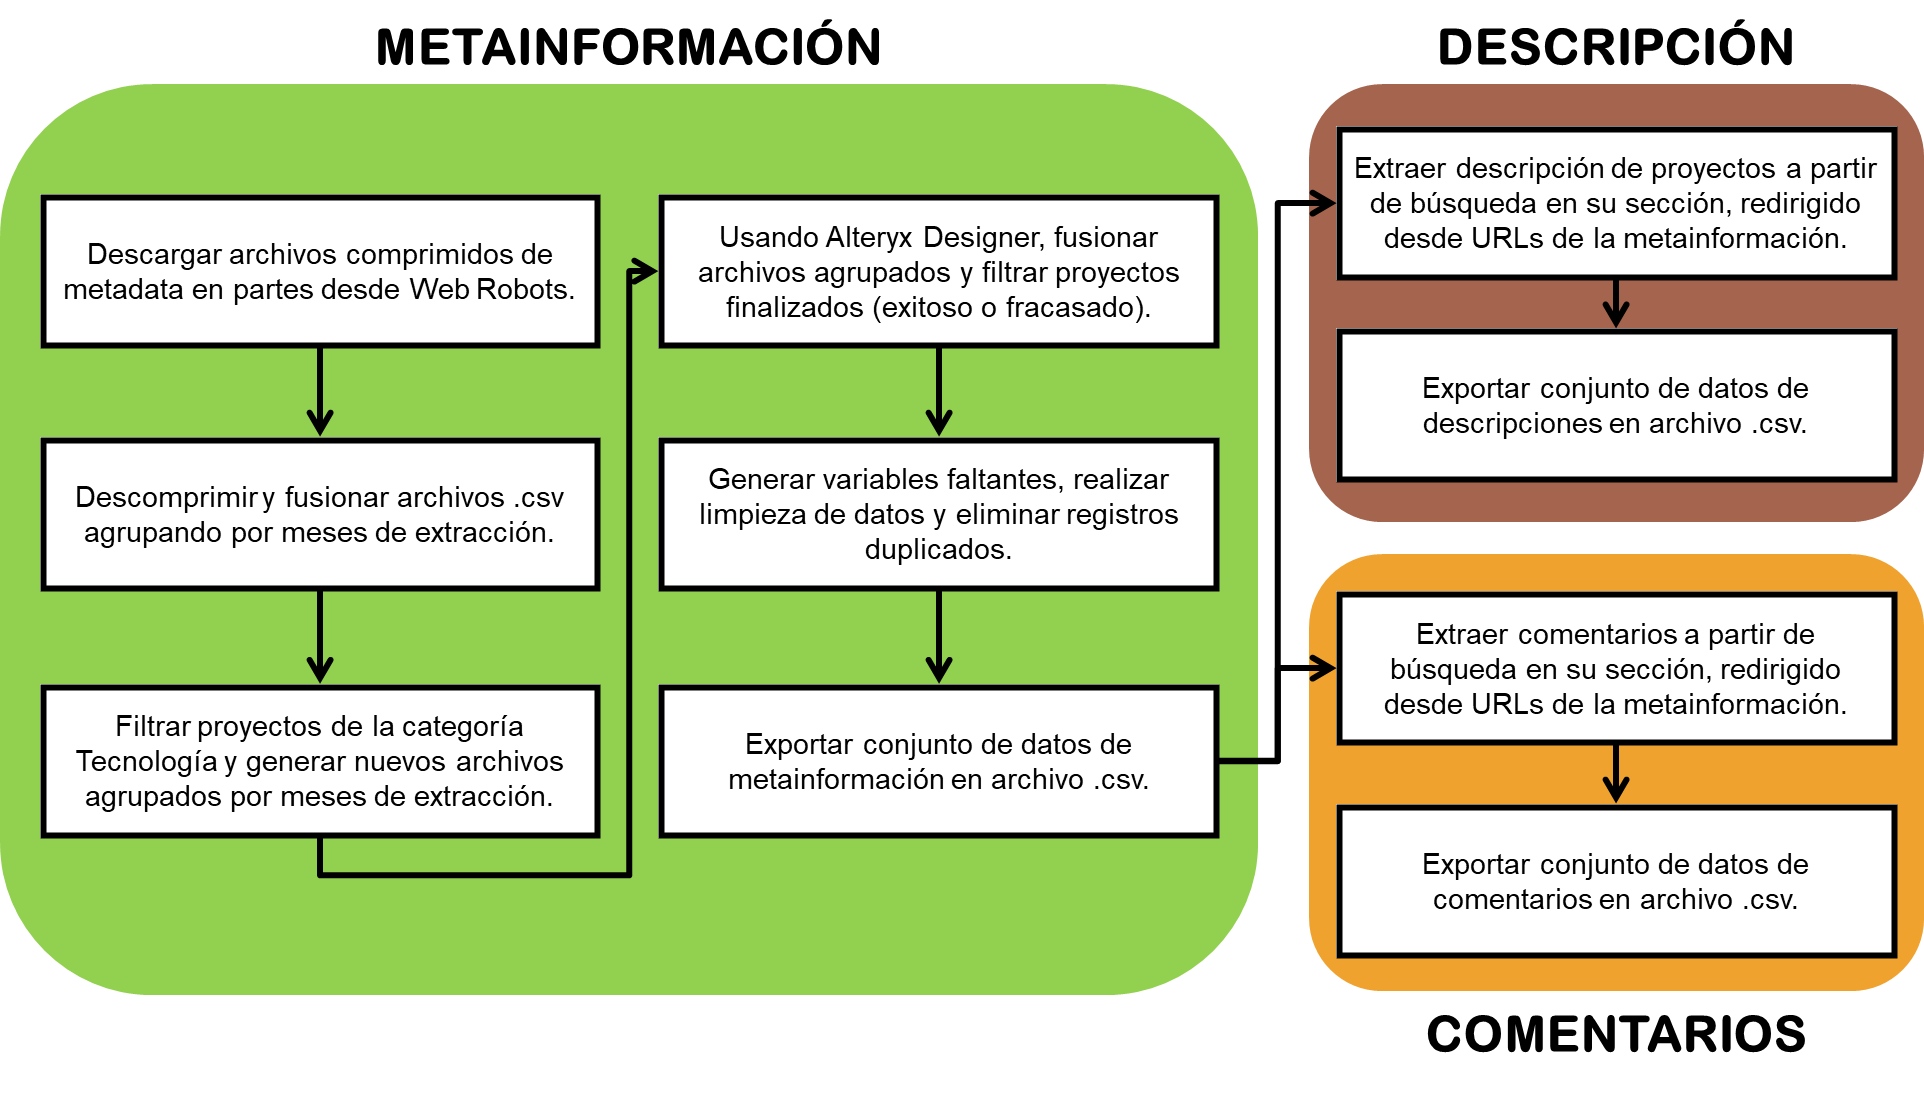
\includegraphics[width=0.89\textwidth]{3/figures/data_recolection_flux.png}
		\caption[Flujograma de la recolección de conjuntos finales de datos]{Flujograma de la recolección de conjuntos finales de datos.\\
			Fuente: Elaboración propia.}
		\label{3:fig1}
	\end{center}
\end{figure}

Asimismo, para encontrar algunos de los papers con la información requerida más cercana, se utilizaron keywords o palabras clave como \textit{crowdfunding}, \textit{Machine Learning}, \textit{Deep Learning}, \textit{prediction}, \textit{Kickstarter}, \textit{accuracy} y \textit{projects}.

%\newpage
\section{Técnicas para el procesamiento y análisis de la información}

\subsection{Metodología de implementación de la solución}
Como se explicó en el punto 2.2.6 del Marco Teórico del presente trabajo, según \cite{tec_braulio2015metodologiasdm}, dentro de los sistemas de analítica de negocio, Big Data y Minería de Datos, tres de las metodologías más usadas son CRISP-DM, SEMMA y KDD. Los mismos autores detallan en la Tabla \ref{2:table1} las características que cada una presenta al compararse.

Para escoger la metodología, se elaboró la Tabla \ref{3:table2} con el fin de comparar las utilizadas por los autores en los antecedentes. 17 de los 18 autores implementaron sus propias metodologías, las cuales de acuerdo a su similitud se agruparon en 8 grupos.

%\newpage
%\begin{table}[htbp]
\vspace{2ex}
\begingroup
	\renewcommand\arraystretch{0.2}
	\begin{longtable}{M{3cm}M{2.5cm}M{2.5cm}M{6cm}}
		\caption[Cuadro comparativo para la selección de la metodología]{Cuadro comparativo para la selección de la metodología.}
		\label{3:table2}
		\newcommand{\multirot}[1]{\multirow{2}{*}[-8ex]{\rotcell{\rlap{#1}}}}
		%\scriptsize
		\footnotesize
		\centering
		\small
		%% Se agrega tabularnewline para longtable
		\tabularnewline \specialrule{.1em}{.05em}{.05em}
		Metodología & Cantidad de referencias & Número de pasos & Nombre de los pasos
		\\
		\specialrule{.1em}{.05em}{.05em}
		{CRISP-DM}
		& 1
		& 6
		& \setlist{nolistsep}
		\begin{itemize}[label={--},nosep,noitemsep,leftmargin=*,topsep=0pt,partopsep=0pt]
			\item Comprensión del negocio.
			\item Comprensión de los datos.
			\item Preparación de los datos.
			\item Modelado.
			\item Evaluación.
			\item Despliegue.
		\end{itemize}                                                 
		\\
		\hline
		{Grupo A}
		& 2
		& 6
		& \setlist{nolistsep}
		\begin{itemize}[label={--},nosep,noitemsep,leftmargin=*,topsep=0pt,partopsep=0pt]
			\item Formulación del problema.
			\item Recolección de datos.
			\item Pre-procesamiento de datos.
			\item Modelado.
			\item Evaluación.
			\item Despliegue.
		\end{itemize} 
		\\
		\hline
		{Grupo B}
		& 1
		& 6
		& \setlist{nolistsep}
		\begin{itemize}[label={--},nosep,noitemsep,leftmargin=*,topsep=0pt,partopsep=0pt]
			\item Formulación del problema.
			\item Recolección de datos.
			\item Selección de características.
			\item Modelado.
			\item Evaluación.
			\item Despliegue.
		\end{itemize} 
		\\
		\hline
		{Grupo C}
		& 2
		& 5
		& \setlist{nolistsep}
		\begin{itemize}[label={--},nosep,noitemsep,leftmargin=*,topsep=0pt,partopsep=0pt]
			\item Recolección de datos.
			\item Pre-procesamiento de datos.
			\item Selección de características.
			\item Modelado.
			\item Evaluación.
		\end{itemize} 
		\\
		\hline
		{Grupo D}
		& 3
		& 5
		& \setlist{nolistsep}
		\begin{itemize}[label={--},nosep,noitemsep,leftmargin=*,topsep=0pt,partopsep=0pt]
			\item Formulación del problema.
			\item Recolección de datos.
			\item Pre-procesamiento de datos.
			\item Modelado.
			\item Evaluación.
		\end{itemize} 
		\\
		\hline
		{Grupo E}
		& 3
		& 5
		& \setlist{nolistsep}
		\begin{itemize}[label={--},nosep,noitemsep,leftmargin=*,topsep=0pt,partopsep=0pt]
			\item Recolección de datos.
			\item Pre-procesamiento de datos.
			\item Modelado.
			\item Evaluación.
			\item Despliegue.
		\end{itemize} 
		\\
		\hline
		{Grupo F}
		& 3
		& 4
		& \setlist{nolistsep}
		\begin{itemize}[label={--},nosep,noitemsep,leftmargin=*,topsep=0pt,partopsep=0pt]
			\item Recolección de datos.
			\item Pre-procesamiento de datos.
			\item Modelado.
			\item Evaluación.
		\end{itemize} 
		\\
		\hline
		{Grupo G}
		& 1
		& 4
		& \setlist{nolistsep}
		\begin{itemize}[label={--},nosep,noitemsep,leftmargin=*,topsep=0pt,partopsep=0pt]
			\item Recolección de datos.
			\item Modelado.
			\item Evaluación.
			\item Despliegue.
		\end{itemize} 
		\\
		\hline
		{Grupo H}
		& 2
		& 3
		& \setlist{nolistsep}
		\begin{itemize}[label={--},nosep,noitemsep,leftmargin=*,topsep=0pt,partopsep=0pt]
			\item Recolección de datos.
			\item Modelado.
			\item Evaluación.
		\end{itemize} 
		\\
		\specialrule{.1em}{.05em}{.05em}
	\end{longtable}%
\endgroup
	%\par	%%Salto de linea
	%\bigskip
	\begin{flushleft}	%%Alinear a la izquierda sin justificar
		\small Fuente: Elaboración propia
	\end{flushleft}
%\end{table}

Si bien es cierto que de las 3 metodologías mencionadas por \citeauthor{tec_braulio2015metodologiasdm}, solamente 1 autor especifica en su investigación el uso de una de ellas, en este caso CRISP-DM \parencite{pr_fernandezblanco2020crowdfunding_empirical}, otros 3 autores (grupos A y B) en sus propias metodologías siguieron secuencias de actividades que se encuentran comprendidas también dentro de esta metodología. Por su parte, los grupos C, F y H guardan cierta relación de semejanza con la metodología SEMMA por comprender enfocarse más en el modeloado, así como tener de primera actividad el Muestreo y culminar con la evaluación de resultados, obviando la actividad de formulación del problema. En el Anexo \ref{anexo4} se puede observar con más detalle las metodologías de la Tabla \ref{3:table2} asignadas a la investigación correspondiente.

Además de lo anterior expuesto, algunas de las siguientes características de acuerdo a la literatura también influyeron en la elección de la metodología CRISP-DM:

\begin{itemize}
	\item La metodología seleccionada contempla entre sus fases la comprensión del negocio además de la parte técnica que incluye el modelado y análisis de resultados. Esta guarda un rol importante ya que en ella se define el inicio de todo el proceso para dar el alcance del proyecto y definir objetivos que se buscan a partir de la Minería de Datos y Big Data. La formulación del problema se encuentra presente en el actual trabajo.
	\item Ayuda a los responsables del proyecto y/o investigación en la planeación y toma de decisiones (fase Despliegue) a partir de los resultados obtenidos, reportando y convirtiéndolos en oportunidades a considerar en los objetivos.
	\item Evalúa en todo el proceso los datos y variables usadas con el fin de crear el mejor modelo. Estas serán importantes para interpretar los resultados y tomar decisiones.
	\item Respecto a las otras dos metodologías, ambas omiten en su primera iteración la formulación del problema, la cual se encuentra presente en el actual trabajo. Por el lado de KDD, si bien esta contempla 9 pasos durante su proceso, el objetivo de KDD en cada uno de estos resulta ser más técnico, es decir, trabajar, seleccionar e interpretar métricas, variables, modelos, entre otros para obtener los mejores resultados más allá de considerar el contexto y comprensión del negocio. De hecho, no existe alguna fase dedicada al entendimiento del mismo.
	\item Por otra parte, la metodología SEMMA se basa, como su nombre lo indica, en la selección, exploración y modelado de grandes cantidades de datos para descubrir patrones de negocio desconocidos. Sin embargo, al limitarse a 5 fases comenzando con la fase de muestreo, no hace hincapié en la comprensión del negocio, sino más bien comienza con el procesamiento de datos para la construcción del modelo.
\end{itemize}

Cada una de las fases de la metodología seleccionada se detalla en la Figura \ref{3:fig2}.

\begin{figure}[htbp]
	\begin{center}
		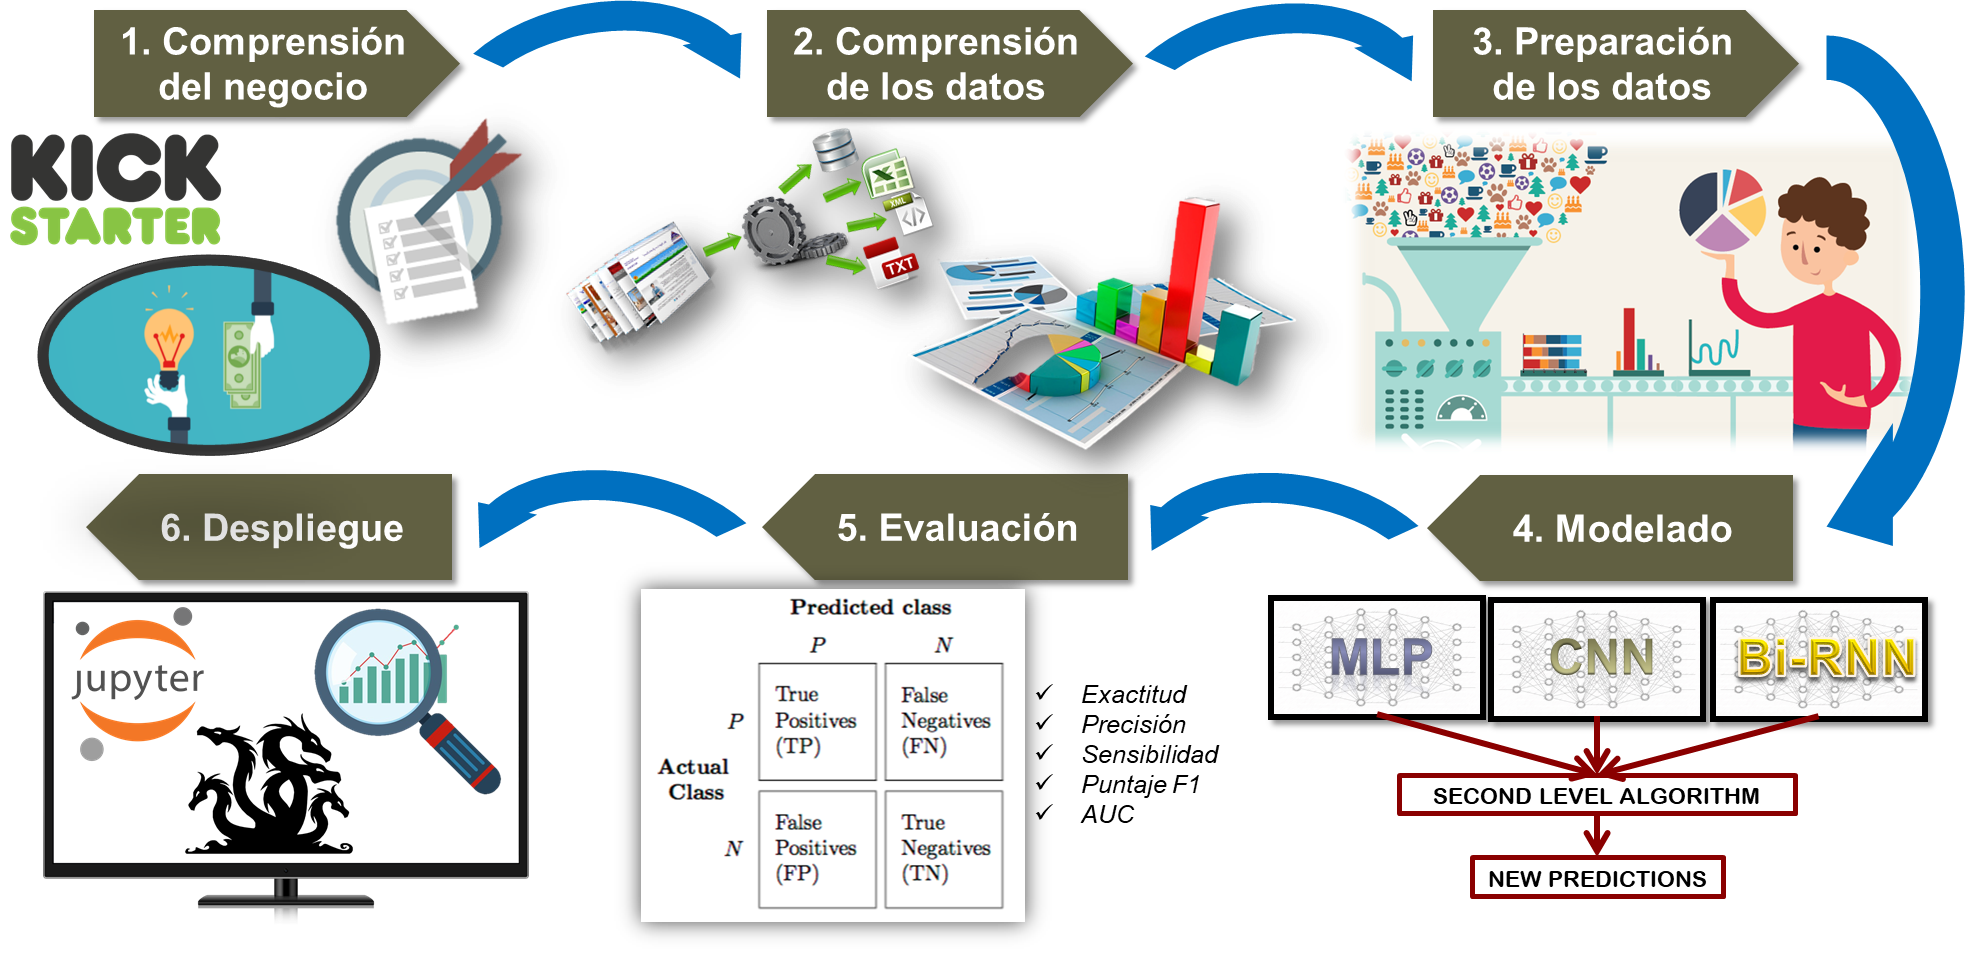
\includegraphics[width=1\textwidth]{3/figures/metodologia.png}
		\caption[Metodología de la investigación]{Metodología de la investigación.\\
			Fuente: Elaboración propia}
		\label{3:fig2}
	\end{center}
\end{figure}

Durante el proceso de la implementación de la metodología, en donde se decidió construir un modelo de Aprendizaje Profundo Multimodal (utilizado por \cite{pr_kamath2018suplearn}, \cite{pr_jin2019dayssuccess}, y \cite{pr_cheng2019deeplearning}), de acuerdo a la literatura, se analizaron las siguientes posibles modalidades que se tomarían en cuenta para la investigación:

\begin{itemize}
	\item \textbf{Metainformación}: \cite{pr_chen2013kickpredict}, \cite{pr_mitra2014phrases}, \cite{pr_zhou2015projectdesc}, \cite{pr_chen2015predcrowd}, \cite{pr_beckwith2016predcrowd}, \cite{pr_li2016predcrowd}, \cite{pr_yuan2016textanalytics}, \cite{pr_sawhney2016usingLT}, \cite{pr_kaur2017socmedcrowd}, \cite{pr_kamath2018suplearn}, \cite{pr_yu2018deeplearning}, \cite{pr_jin2019dayssuccess}, \cite{pr_cheng2019deeplearning}, \cite{pr_fernandezblanco2020crowdfunding_empirical}.
	\item \textbf{Descripción del proyecto}: \cite{pr_mitra2014phrases}, \cite{pr_zhou2015projectdesc}, \cite{pr_yuan2016textanalytics}, \cite{pr_sawhney2016usingLT}, \cite{pr_kamath2018suplearn}, \cite{pr_lee2018contentDL}, \cite{pr_jin2019dayssuccess}, \cite{pr_cheng2019deeplearning}, \cite{pr_chen2019keywords_crowdfunding}, \cite{pr_chaichi2019nlp_3dprinting}.
	\item \textbf{Comentarios en la campaña}: \cite{pr_chen2015predcrowd}, \cite{pr_li2016predcrowd}, \cite{pr_lee2018contentDL}, \cite{pr_jin2019dayssuccess}, \cite{pr_shafqat2019topicpredictions}.
	\item \textbf{Actualizaciones y/o recompensas}: \cite{pr_zhou2015projectdesc}, \cite{pr_lee2018contentDL}.
	\item \textbf{Contenido audiovisual (imagen y/o video del proyecto)}: \cite{pr_cheng2019deeplearning}.
\end{itemize}

De las anteriores modalidades, las actualizaciones no representan un cambio significativo ya que consisten en agregar o desagregar contenido textual o modificar recompensas en la campaña. Por el lado del contenido audiovisual, además de no presentarse en todas las campañas, para el caso particular de la categoría Tecnología no se encontró un patrón entre sus imágenes que pueda ser de utilidad, como se presenta en el trabajo de tesis de pregrado del presente investigador \parencite{pr_puente2019kickstarter_prediction}.

Finalmente, fueron seleccionadas las modalidades de metainformación, descripción del proyecto y comentarios, para este último considerando solamente expresados por patrocinadores. Las 2 primeras se localizan en la sección principal de la campaña, mientras que la tercera se ubica en su sección respectiva, como se puede apreciar en la Figura \ref{3:fig3}.
\begin{figure}[htbp]
	\begin{center}
		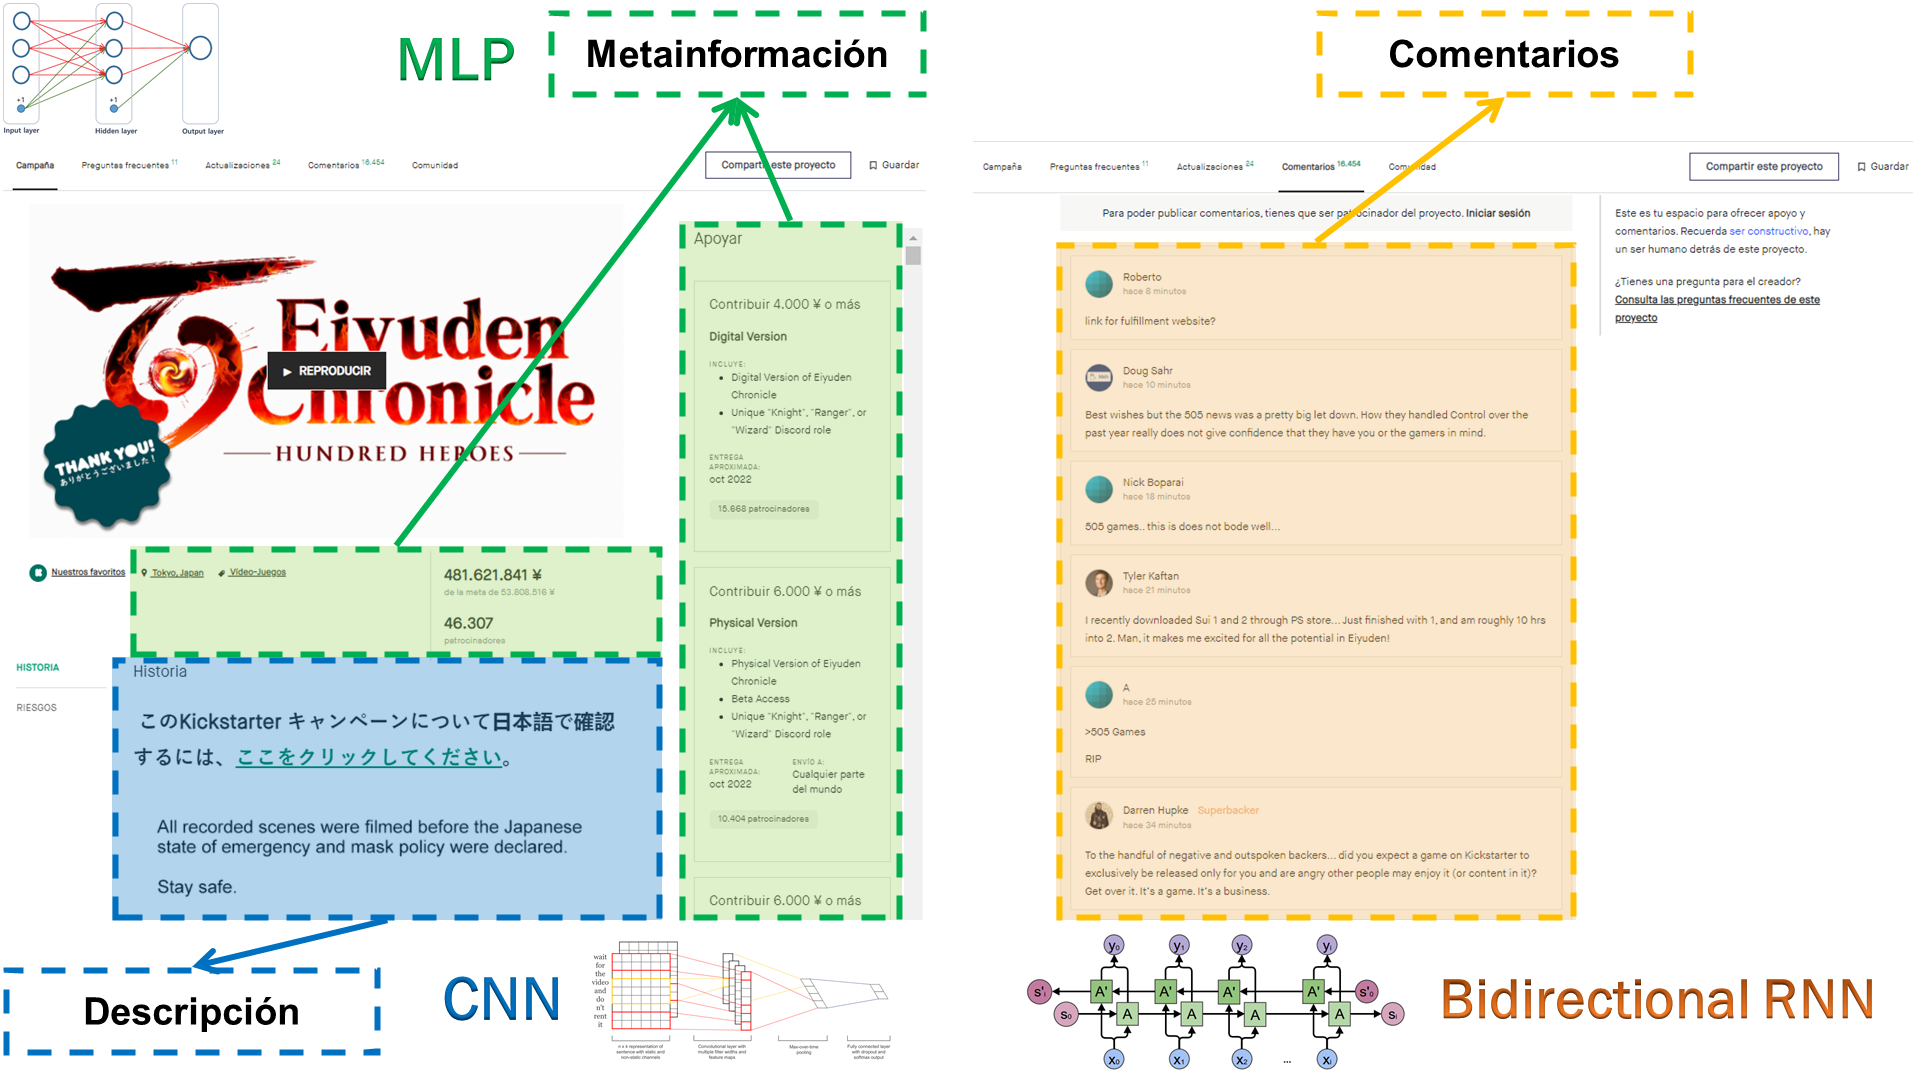
\includegraphics[width=0.90\textwidth]{3/figures/framework.png}
		\caption[Marco de trabajo del prototipo final]{Marco de trabajo del prototipo final.\\
			Fuente: Elaboración propia}
		\label{3:fig3}
	\end{center}
\end{figure}

\newpage
\subsubsection{Comprensión del negocio}
En la primera fase, se definió el problema a partir de comprender el contexto de la investigación. A partir de aquí, se formularon los objetivos y requerimientos que se espera lograr en el proyecto. La lista de actividades y tareas se presenta en la Tabla \ref{3:table3}.

\vspace{2ex}
\begingroup
\renewcommand\arraystretch{0.3}
\begin{longtable}{m{5cm}m{5cm}M{5cm}}
	\caption[Actividades de fase Comprensión del negocio]{Actividades de fase Comprensión del negocio.}
	\label{3:table3}
	\newcommand{\multirot}[1]{\multirow{2}{*}[-8ex]{\rotcell{\rlap{#1}}}}
	%\scriptsize
	\footnotesize
	%\centering
	\small
	%% Se agrega tabularnewline para longtable
	\tabularnewline \specialrule{.1em}{.05em}{.05em}
	\centering Actividades & \centering Descripción & Tareas
	\\
	\specialrule{.1em}{.05em}{.05em}
	Definir problemas, objetivos e hipótesis.
	& Definición de los problemas, objetivos e hipótesis generales y específicos de la investigación.
	& \setlist{nolistsep}
	\begin{itemize}[label={--},nosep,noitemsep,leftmargin=*,topsep=0pt,partopsep=0pt]
		\item Identificar la realidad problemática del contexto.
		\item Definir los objetivos de la investigación.
		\item Formular las hipótesis del trabajo.
	\end{itemize}                                               
	\\
	\hline
	Desarrollar la literatura de la investigación.
	& Selección de los antecedentes y trabajos previos relacionados a la investigación.
	& \setlist{nolistsep}
	\begin{itemize}[label={--},nosep,noitemsep,leftmargin=*,topsep=0pt,partopsep=0pt]
		\item Buscar material académico sobre las variables de la investigación.
		\item Buscar material académico relacionado a la solución de la realidad problemática.
	\end{itemize} 
	\\
	\hline
	Definir metodología de la investigación.
	& Definición de la metodología a implementarse en el estudio.
	& \setlist{nolistsep}
	\begin{itemize}[label={--},nosep,noitemsep,leftmargin=*,topsep=0pt,partopsep=0pt]
		\item Evaluar metodologías de la literatura.
		\item Seleccionar metodología a implementar en el trabajo.
	\end{itemize} 
	\\
	\specialrule{.1em}{.05em}{.05em}
\end{longtable}%
\endgroup

%\par	%%Salto de linea
%\bigskip
\begin{flushleft}	%%Alinear a la izquierda sin justificar
	\small Fuente: Elaboración propia
\end{flushleft}

A continuación, cada actividad de la anterior tabla es detallada y se indican sus entregables respectivos.

\newpage
\textbf{Actividad 1: Definir problemas, objetivos e hipótesis}
\\
En esta actividad se detalla cómo se definieron los problemas, objetivos e hipótesis generales y específicos de la investigación a partir del estudio de la coyuntura en que se desenvuelve la realidad problemática.

\textbf{Entregable}: Problemas, objetivos e hipótesis definidos.


\textbf{Actividad 2: Desarrollar la literatura de la investigación}
\\
A partir de la definición de los objetivos, se realizó la búsqueda de fuentes, publicaciones, libros, artículos y material académico relacionado al contexto del financiamiento colectivo, sus características y qué métodos se utilizaron para resolver problemas dentro del entorno. Asimismo, se elaboró el marco teórico abordado en el estudio.

\textbf{Entregable}: Material académico y conocimientos obtenidos sobre el ambiente del crowdfunding y la Inteligencia Artificial.


\textbf{Actividad 3: Definir metodología de la investigación}
\\
Luego de conseguir los recursos intelectuales suficientes y los trabajos previos para el desarrollo de la investigación, se analizó cada antecedente y se compararon todas las metodologías implementadas por cada autor. Al culminar con esta tarea, en base a la literatura y los procesos más alineados al presente trabajo, se seleccionó la metodología CRISP-DM como la mejor opción.

\textbf{Entregable}: Metodología de implementación de la solución.


\subsubsection{Comprensión de los datos}
La segunda fase abarcó tanto la recolección de los datos como el análisis estadístico de estos para conocer un poco más sus características. El conjunto total de datos utilizado para la investigación consistió en la recolección de 27,251 proyectos tecnológicos de Kickstarter comprendidos entre los años 2009 y 2019, en 3 partes: metainformación, descripción y comentarios (excluyendo los del creador) del proyectos.

Para ello, se elaboró una lista de actividades y tareas presentadas en la Tabla \ref{3:table4}.

\vspace{2ex}
\begingroup
\renewcommand\arraystretch{0.3}
\begin{longtable}{m{4cm}m{5.5cm}M{5.5cm}}
	\caption[Actividades de fase Comprensión de los datos]{Actividades de fase Comprensión de los datos.}
	\label{3:table4}
	\newcommand{\multirot}[1]{\multirow{2}{*}[-8ex]{\rotcell{\rlap{#1}}}}
	%\scriptsize
	\footnotesize
	%\centering
	\small
	%% Se agrega tabularnewline para longtable
	\tabularnewline \specialrule{.1em}{.05em}{.05em}
	\centering Actividades & \centering Descripción & Tareas
	\\
	\specialrule{.1em}{.05em}{.05em}
	Construir base de datos de Metainformación.
	& Construcción de base de datos que contenga las variables de la campaña con excepción del contenido textual (descripción, actualizaciones y comentarios acerca del proyecto).
	& \setlist{nolistsep}
	\begin{itemize}[label={--},nosep,noitemsep,leftmargin=*,topsep=0pt,partopsep=0pt]
		\item Descargar conjuntos de datos comprimidos de la página Web Robots.
		\item Descomprimir archivos en partes y fusionarlos en uno solo según su mes.
		\item Fusionar archivos por mes, realizar limpieza de datos y generar base final.
	\end{itemize} 
	\\
	\hline
	Construir base de datos de Descripción.
	& Construcción de base de datos que contenga la descripción del proyecto en la página principal de la campaña.
	& \setlist{nolistsep}
	\begin{itemize}[label={--},nosep,noitemsep,leftmargin=*,topsep=0pt,partopsep=0pt]
		\item Identificar sección de descripción a partir de la búsqueda del URL desde la base de datos de Metainformación.
		\item Capturar información de sección identificada.
		\item Generar base final.
	\end{itemize} 
	\\
	\hline
	Construir base de datos de Comentarios.
	& Construcción de base de datos que contenga los comentarios de los patrocinadores del proyecto en su sección correspondiente.
	& \setlist{nolistsep}
	\begin{itemize}[label={--},nosep,noitemsep,leftmargin=*,topsep=0pt,partopsep=0pt]
		\item Identificar sección de comentarios a partir de la búsqueda del URL desde la base de datos de Metainformación.
		\item Capturar información de sección identificada, excluyendo comentarios y respuestas de los creadores del proyecto.
		\item Generar base final.
	\end{itemize}
	\\
	\hline
	Realizar análisis exploratorio y estadístico de variables considerados.
	& Análisis exploratorio y estadístico de las variables disponibles para cada modalidad.
	& \setlist{nolistsep}
	\begin{itemize}[label={--},nosep,noitemsep,leftmargin=*,topsep=0pt,partopsep=0pt]
		\item Describir distribución de los datos y tendencias.
		\item Analizar existencia de correlación entre variables.
	\end{itemize}
	\\
	\specialrule{.1em}{.05em}{.05em}
\end{longtable}%
\endgroup

%\par	%%Salto de linea
%\bigskip
\begin{flushleft}	%%Alinear a la izquierda sin justificar
	\small Fuente: Elaboración propia
\end{flushleft}

A continuación, se detalla cada actividad y su entregable respectivo.

\textbf{Actividad 1: Construir base de datos de Metainformación}
\\
De acuerdo a la Figura \ref{3:fig1}, en esta actividad se enfocó en la construcción de la base de datos de la Metainformación desde la descarga de los conjuntos de datos comprimidos de la página Web Robots hasta la generación del archivo final luego de limpiar los datos.

La 2 primeras tareas de la anterior tabla se resumen en el flujo de la Figura \ref{3:fig4}.

\begin{figure}[h]
	\begin{center}
		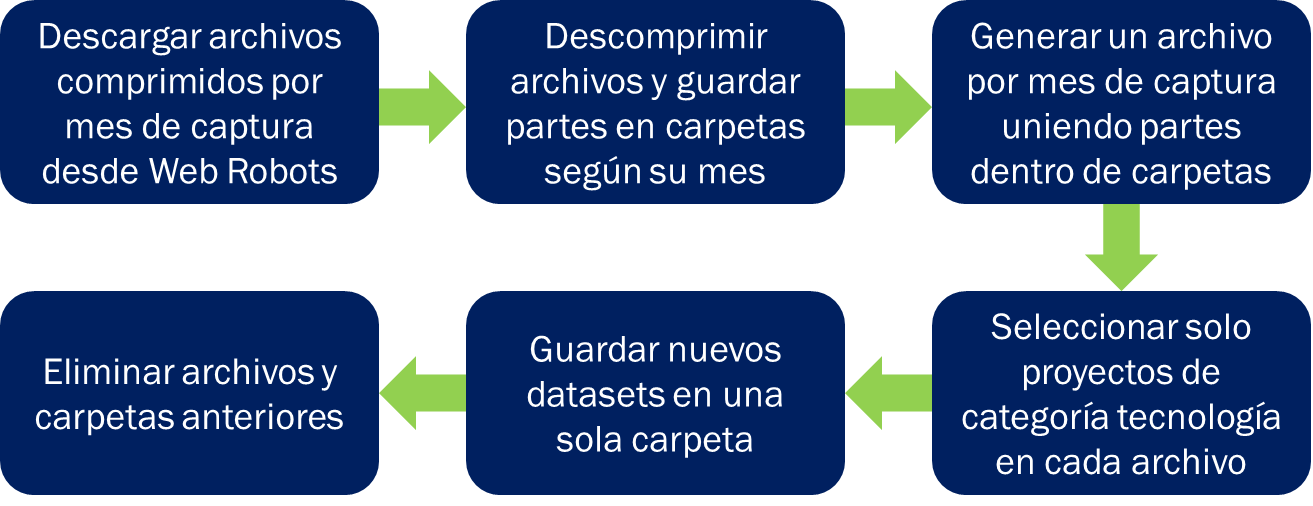
\includegraphics[width=0.8\textwidth]{3/figures/flujograma_metadata_t1_t2.png}
		\caption[Proceso de obtención y preparación de datasets iniciales de Metainformación]{Proceso de obtención y preparación de datasets iniciales de Metainformación.\\
			Fuente: Elaboración propia.}
		\label{3:fig4}
	\end{center}
\end{figure}

La siguiente fase de la actividad fue la selección de variables y limpieza de datos utilizando el software Alteryx Designer, el cual permite desarrollar flujos de trabajo para preparar, unir y analizar volúmenes de datos complejos de distintas fuentes. Se ejecutó el flujograma representado de forma resumida en la Figura \ref{3:fig5}.

\begin{figure}[h]
	\begin{center}
		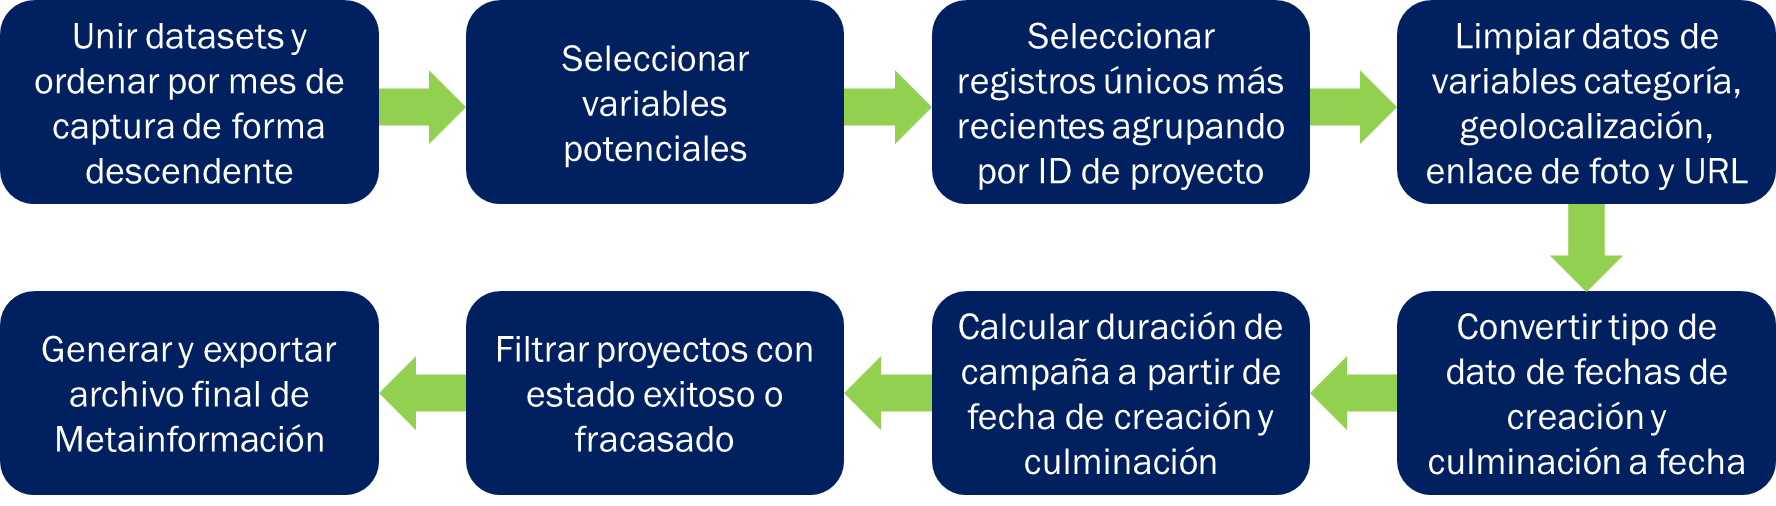
\includegraphics[width=1\textwidth,clip]{3/figures/flujograma_metadata_t3.png}
		\caption[Proceso resumido de generación de conjunto final de Metainformación]{Proceso resumido de generación de conjunto final de Metainformación.\\
			Fuente: Elaboración propia.}
		\label{3:fig5}
	\end{center}
\end{figure}

\textbf{Entregable}: Conjunto de datos de Metainformación, que contiene 19 variables cuantitativas y cualitativas para la muestra considerada.

\textbf{Actividad 2: Construir base de datos de Descripción}
\\
De acuerdo a la Figura \ref{3:fig1}, una vez generado el conjunto de datos de Metainformación descrito en la anterior actividad, a partir de la variable \textit{urls} se puede extraer la descripción de cada proyecto, siguiendo el proceso del diagrama de flujo representado en la Figura \ref{3:fig6}.

\begin{figure}[h]
	\begin{center}
		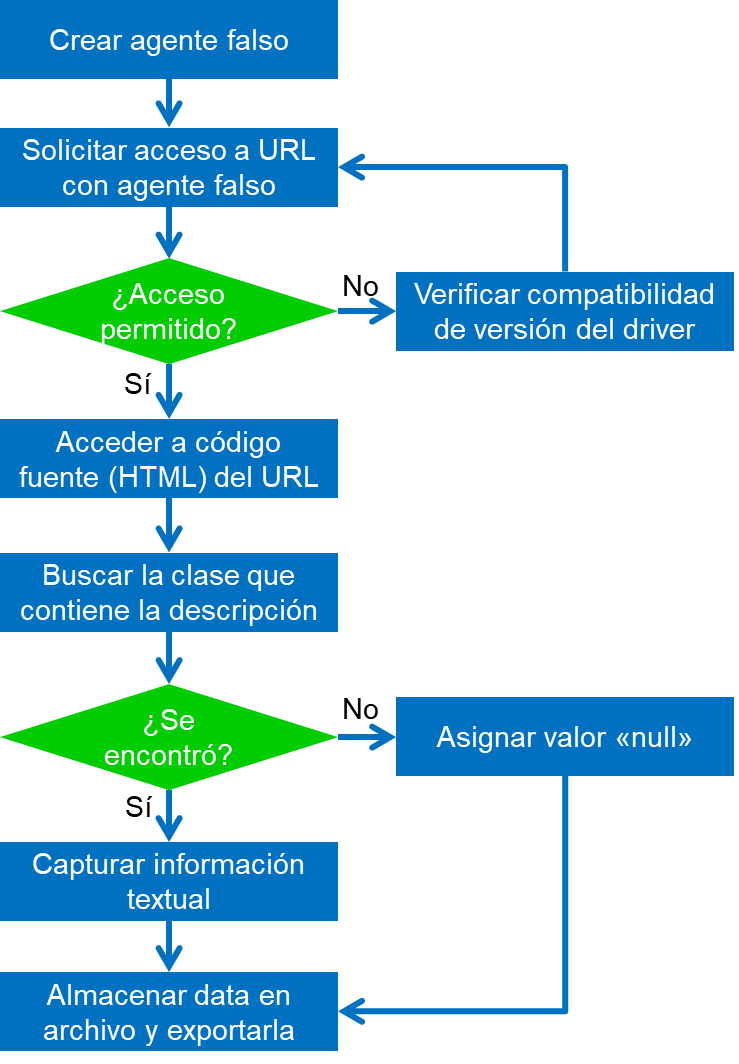
\includegraphics[width=0.5\textwidth]{3/figures/diagrama_flujo_scrapping_descripcion.png}
		\caption[Proceso de extracción de la descripción de un proyecto]{Proceso de extracción de la descripción de un proyecto.\\
			Fuente: Elaboración propia.}
		\label{3:fig6}
	\end{center}
\end{figure}

\textbf{Entregable}: Conjunto de datos de Descripción, que contiene la variable textual de descripción del proyecto para la muestra considerada.

\textbf{Actividad 3: Construir base de datos de Comentarios}
\\
De acuerdo a la Figura \ref{3:fig1}, y realizando el mismo ejercicio con Descripción, una vez generado el conjunto de datos de Metainformación, a partir de la variable \textit{urls} se pueden extraer los comentarios de los patrocinadores por cada proyecto, siguiendo el proceso del diagrama de flujo representado en la Figura \ref{3:fig7}.

\begin{figure}[h]
	\begin{center}
		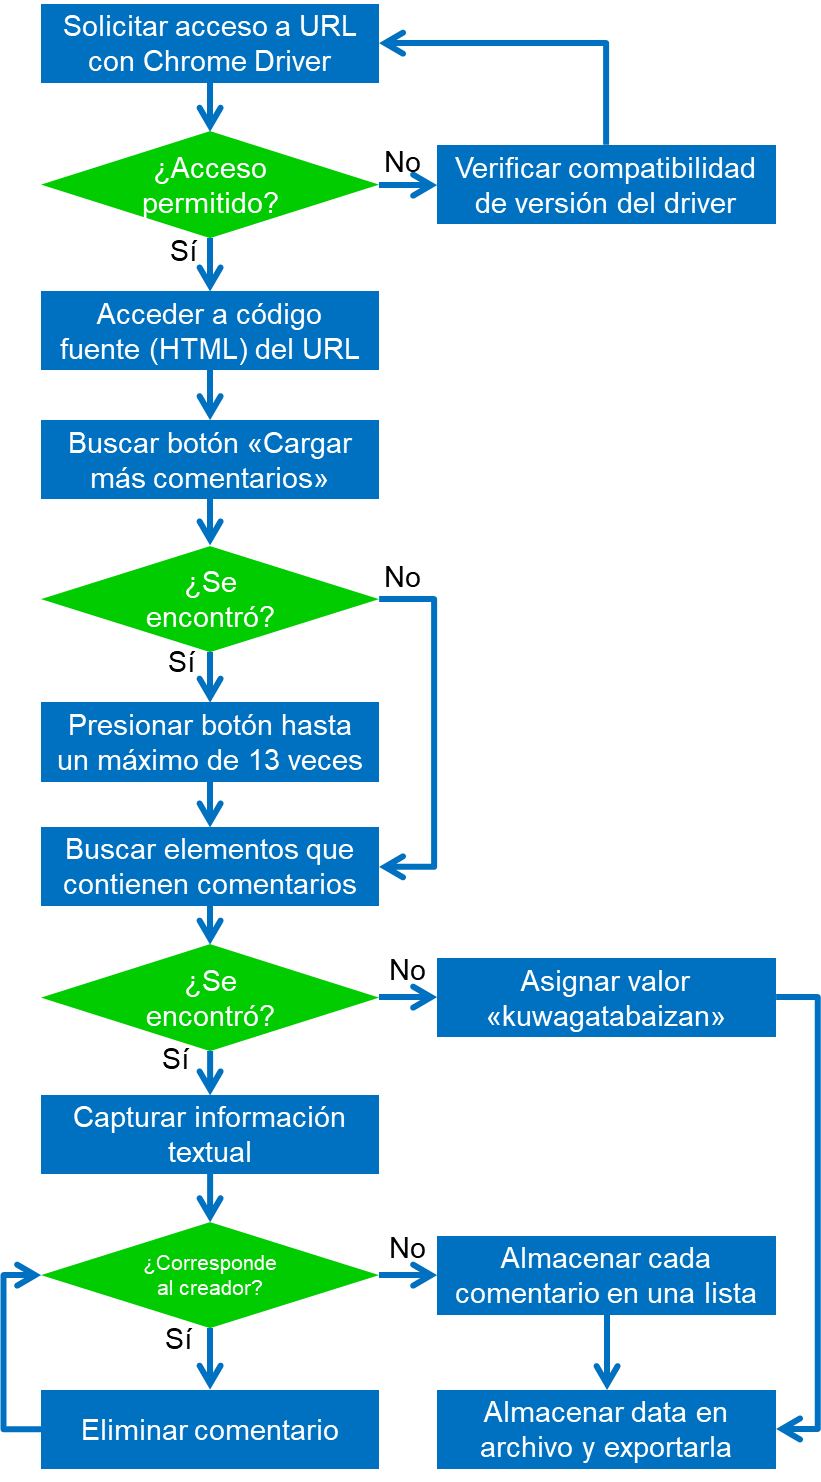
\includegraphics[width=0.45\textwidth]{3/figures/diagrama_flujo_scrapping_comentarios.png}
		\caption[Proceso de extracción de comentarios de un proyecto]{Proceso de extracción de comentarios de un proyecto.\\
			Fuente: Elaboración propia.}
		\label{3:fig7}
	\end{center}
\end{figure}

\textbf{Entregable}: Conjunto de datos de Comentarios, que contiene la variable textual de comentarios de los patrocinadores, cada uno separado por autor y almacenados en conjunto en una lista por proyecto, para la muestra considerada.

\textbf{Actividad 4: Realizar análisis exploratorio y estadístico de variables considerados}
\\
En esta actividad, las variables de los 3 conjuntos finales de datos se describen en distribución de gráficos de barras, diagramas de cajas y bigotes y análisis de correlaciones de variables para la Metainformación; y nubes de palabras para la Descripción y Comentarios.

\textbf{Entregable}: Gráficos estadísticos de Metainformación, Descripción y Comentarios.

\subsubsection{Preparación de los datos}
En el anterior paso, se logró analizar estadísticamente las tendencias y distribuciones de cada variable según su respectiva modalidad. En esta etapa, como se detalla en la Tabla \ref{3:table5}, las variables observadas fueron pre-procesadas con la finalidad de incluir datos homologados que no afecten negativamente el rendimiento de los modelos.

\vspace{2ex}
\begingroup
\renewcommand\arraystretch{0.3}
\begin{longtable}{m{5cm}m{5cm}M{5cm}}
	\caption[Actividades de fase Preparación de los datos]{Actividades de fase Preparación de los datos.}
	\label{3:table5}
	\newcommand{\multirot}[1]{\multirow{2}{*}[-8ex]{\rotcell{\rlap{#1}}}}
	%\scriptsize
	\footnotesize
	%\centering
	\small
	%% Se agrega tabularnewline para longtable
	\tabularnewline \specialrule{.1em}{.05em}{.05em}
	\centering Actividades & \centering Descripción & Tareas
	\\
	\specialrule{.1em}{.05em}{.05em}
	Pre-procesar base de datos de Metainformación.
	& Pre-procesamiento de las variables actuales y adicionales luego de evaluación de su comportamiento entre ellas.
	& \setlist{nolistsep}
	\begin{itemize}[label={--},nosep,noitemsep,leftmargin=*,topsep=0pt,partopsep=0pt]
		\item Añadir más variables cuantitativas según literatura.
		\item Evaluar comportamiento de variables en conjunto utilizando matriz de correlaciones.
		\item Armar grupos combinatorias potenciales de variables.
		\item Escalar variables a un mismo rango.
	\end{itemize}                                             
	\\
	\hline
	Pre-procesar base de datos de Descripción.
	& Pre-procesamiento de la variable \textit{description}.
	& \setlist{nolistsep}
	\begin{itemize}[label={--},nosep,noitemsep,leftmargin=*,topsep=0pt,partopsep=0pt]
		\item Realizar limpieza de datos de los textos.
		\item Armar vocabulario de palabras únicas.
		\item Transformar textos en vectores de palabras.
	\end{itemize} 
	\\
	\hline
	Pre-procesar base de datos de Comentarios.
	& Pre-procesamiento de la variable \textit{comments}.
	& \setlist{nolistsep}
	\begin{itemize}[label={--},nosep,noitemsep,leftmargin=*,topsep=0pt,partopsep=0pt]
		\item Realizar limpieza de datos de los textos.
		\item Armar vocabulario de palabras únicas.
		\item Transformar textos en vectores de palabras.
	\end{itemize}
	\\
	\specialrule{.1em}{.05em}{.05em}
\end{longtable}%
\endgroup

%\par	%%Salto de linea
%\bigskip
\begin{flushleft}	%%Alinear a la izquierda sin justificar
	\small Fuente: Elaboración propia
\end{flushleft}

A continuación, se detalla cada actividad y su entregable respectivo.

\textbf{Actividad 1: Pre-procesar base de datos de Metainformación}
\\
En esta actividad, antes de realizar el pre-procesamiento de las variables finales, se agregaron algunas cuantitativas sugeridas en la literatura que no estaban consideradas inicialmente. Para evaluar correctamente el nuevo conjunto de variables, se realizó un nuevo análisis de correlación y se armaron grupos de combinatorias de variables cuyos rendimientos serán medidos en los siguientes pasos. Previamente a la evaluación, los subconjuntos de entrenamiento y prueba divididos en 80\% y 20\% respectivamente (según \cite{pr_yuan2016textanalytics}, \cite{pr_yu2018deeplearning}, \cite{pr_chen2019keywords_crowdfunding}, \cite{pr_mitra2014phrases} y \cite{pr_sawhney2016usingLT}) estratificados según la variable \textit{state}, se escalaron a un mismo rango para evitar un entrenamiento incorrecto.

\textbf{Entregable}: Conjuntos de datos pre-procesados de Metainformación.

\textbf{Actividad 2: Pre-procesar base de datos de Descripción}
\\
Esta actividad se resume en la Figura \ref{3:fig8}, en donde se realizó desde la limpieza de los datos textuales, eliminando palabras y partes de ellas que no aportan para el diccionario final que se usará en la siguiente etapa, hasta la elaboración del vocabulario de palabras únicas, mayormente sustantivos y verbos en su forma original, los cuales se les asignaron un código para poder formar vectores de palabras y crear más adelante, las incrustaciones de palabras.

\begin{figure}[!ht]
	\begin{center}
		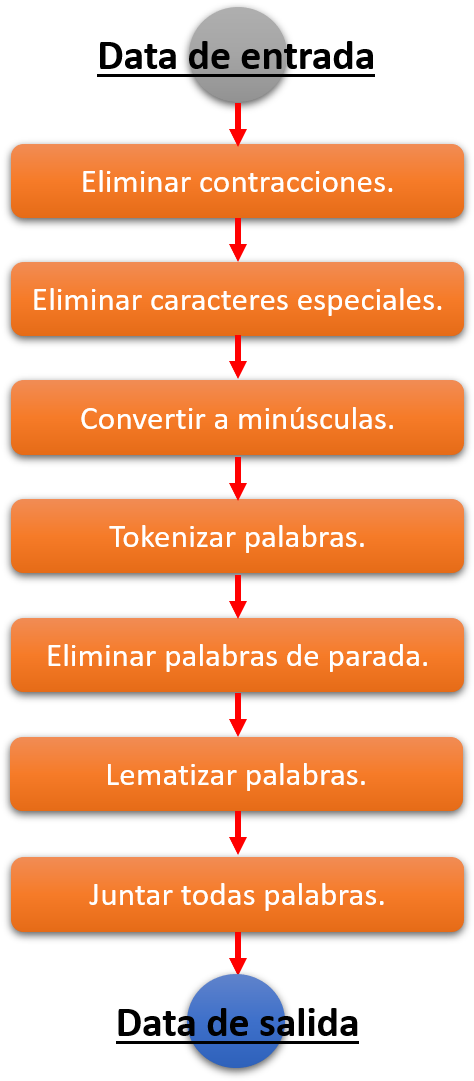
\includegraphics[width=0.33\textwidth]{3/figures/description_data_clean.png}
		\caption[Proceso de limpieza de conjunto de datos de descripciones]{Proceso de limpieza de conjunto de datos de descripciones.\\
			Fuente: Elaboración propia.}
		\label{3:fig8}
	\end{center}
\end{figure}

Luego de separar, al igual que la Metainformación, los subconjuntos de entrenamiento y prueba en 80\% y 20\% respectivamente estratificados según la variable \textit{state}, se ejecutó el proceso de la Figura \ref{3:fig9} dividido en 2 partes.

\begin{figure}[!ht]
	\centering
	\small
	\begin{subfigure}{.50\textwidth}
		\centering
		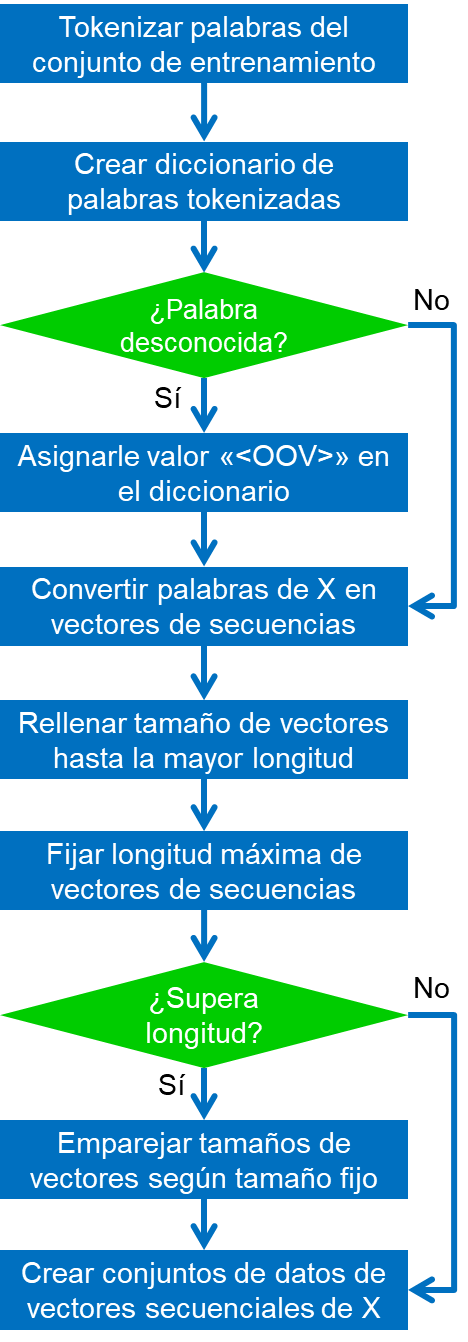
\includegraphics[width=0.65\linewidth]{3/figures/description_text_to_sequence.png}
		\caption{vectorización de palabras}
	\end{subfigure}%
	\begin{subfigure}{.50\textwidth}
		\centering
		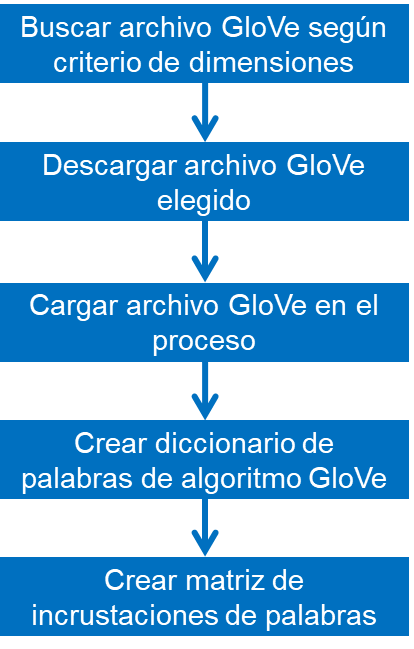
\includegraphics[width=0.55\linewidth]{3/figures/description_embedding_matrix.png}
		\caption{matriz de incrustaciones de palabras}
	\end{subfigure}
	\caption[Procesos de vectorización y creación de matriz incrustaciones de palabras]{Procesos de vectorización y creación de matriz incrustaciones de palabras.\\
		Fuente: Elaboración propia.}
	\label{3:fig9}
\end{figure}

La primera mitad corresponde a la transformación del texto, para los subconjuntos de entrenamiento y prueba, de las descripciones en representaciones de vectores numéricos para la fase de entrenamiento del modelo. De forma paralela, se creó una matriz de incrustaciones de palabras que será parte de la capa de incrustaciones en la arquitectura del modelo.

\textbf{Entregable}: Descripciones representadas en secuencias de vectores numéricos y matriz de incrustaciones de palabras.

\textbf{Actividad 3: Pre-procesar base de datos de Comentarios}
\\
Al igual que en el proceso de Descripción, se realizó la limpieza de los datos textuales siguiendo la misma secuencia de la Figura \ref{3:fig7} para generar la representación de palabras de los comentarios en vectores numéricos, con la diferencia de acotar el tamaño final de los vectores debido a su extensa longitud al agruparse todos aquellos separados por autor. De igual manera, para generar la matriz de incrustaciones de palabras, se repitió el proceso de la Figura \ref{3:fig9}.

\textbf{Entregable}: Comentarios representadas en secuencias de vectores numéricos y matriz de incrustaciones de palabras.

\subsubsection{Modelamiento}
Al concluir la etapa del pre-procesamiento, las variables pudieron ser utilizadas para los modelos de cada modalidad, que fueron diseñados siguiendo las actividades de la Tabla \ref{3:table6}.

\vspace{2ex}
\begingroup
\renewcommand\arraystretch{0.3}
\begin{longtable}{m{4.6cm}m{4.9cm}M{5.5cm}}
	\caption[Actividades de fase Modelamiento]{Actividades de fase Modelamiento.}
	\label{3:table6}
	\newcommand{\multirot}[1]{\multirow{2}{*}[-8ex]{\rotcell{\rlap{#1}}}}
	%\scriptsize
	\footnotesize
	% \centering
	\small
	%% Se agrega tabularnewline para longtable
	\tabularnewline \specialrule{.1em}{.05em}{.05em}
	\centering Actividades & \centering Descripción & Tareas
	\\
	\specialrule{.1em}{.05em}{.05em}
	Desarrollar modelo predictivo de Metainformación.
	& Implementación del modelo Perceptrón Multicapa (MLP) para la modalidad Metainformación.
	& \setlist{nolistsep}
	\begin{itemize}[label={--},nosep,noitemsep,leftmargin=*,topsep=0pt,partopsep=0pt]
		\item Realizar benchmarking de modelos utilizados en trabajos previos.
		\item Diseñar arquitectura del modelo predictivo de acuerdo a opción escogida.
	\end{itemize}
	\\
	\hline
	Desarrollar modelo predictivo de Descripción.
	& Implementación de la Red Neuronal Convolucional (CNN) para la modalidad Descripción.
	& \setlist{nolistsep}
	\begin{itemize}[label={--},nosep,noitemsep,leftmargin=*,topsep=0pt,partopsep=0pt]
		\item Realizar benchmarking de modelos utilizados en trabajos previos.
		\item Diseñar arquitectura del modelo predictivo de acuerdo a opción escogida.
	\end{itemize}
	\\
	\hline
	Desarrollar modelo predictivo de Comentarios.
	& Implementación del modelo LSTM Bidireccional para la modalidad Comentarios.
	& \setlist{nolistsep}
	\begin{itemize}[label={--},nosep,noitemsep,leftmargin=*,topsep=0pt,partopsep=0pt]
		\item Realizar benchmarking de modelos utilizados en trabajos previos.
		\item Diseñar arquitectura del modelo predictivo de acuerdo a opción escogida.
	\end{itemize}
	\\
	\hline
	Desarrollar modelo ensamblado apilado.
	& Implementación del modelo de Aprendizaje Profundo Multimodal.
	& \setlist{nolistsep}
	\begin{itemize}[label={--},nosep,noitemsep,leftmargin=*,topsep=0pt,partopsep=0pt]
		\item Realizar benchmarking de modalidades utilizadas en trabajos previos.
		\item Diseñar arquitectura del modelo ensamblado apilado.
	\end{itemize}
	\\
	\specialrule{.1em}{.05em}{.05em}
\end{longtable}%
\endgroup
%\par	%%Salto de linea
%\bigskip
\begin{flushleft}	%%Alinear a la izquierda sin justificar
	\small Fuente: Elaboración propia
\end{flushleft}

%A continuación, se detalla cada actividad y su entregable respectivo.
\textbf{Actividad 1: Desarrollar modelo predictivo de Metainformación}
\\
En esta actividad, se diseñó la arquitectura que se usó para la modalidad Metainformación. Para ello, se realizó benchmarking sobre las propuestas de los autores enunciadas a continuación.

\begin{itemize}
	\item \textbf{Perceptrón Multicapa (MLP)}: \cite{pr_kamath2018suplearn}, \cite{pr_yu2018deeplearning}, \cite{pr_cheng2019deeplearning}.
	\item \textbf{Máquina de Vectores de Soporte (SVM)}: \cite{pr_chen2013kickpredict}, \cite{pr_beckwith2016predcrowd}, \cite{pr_sawhney2016usingLT}.
	\item \textbf{Regresión Logística}: \cite{pr_mitra2014phrases}, \cite{pr_zhou2015projectdesc}, \cite{pr_beckwith2016predcrowd}, \cite{pr_li2016predcrowd}, \cite{pr_kaur2017socmedcrowd}.
	\item \textbf{Regresión Log-logística}: \cite{pr_li2016predcrowd}.
	\item \textbf{Bosques Aleatorios}: \cite{pr_chen2015predcrowd}, \cite{pr_yuan2016textanalytics}, \cite{pr_kamath2018suplearn}.
	\item \textbf{Árboles de Decisión}: \cite{pr_beckwith2016predcrowd}, \cite{pr_kamath2018suplearn}.
	\item \textbf{Naïve Bayes}: \cite{pr_beckwith2016predcrowd}, \cite{pr_kamath2018suplearn}.
	\item \textbf{Modelo Seq2seq}: \cite{pr_jin2019dayssuccess}.
\end{itemize}

De acuerdo a los resultados de los autores citados, los modelos de Redes Neuronales (MLP), SVM y Regresión Logística tuvieron los mejores rendimientos en sus experimentos. Dado que la investigación consistió en implementar un modelo de Aprendizaje Profundo Multimodal, en donde se ensamblan modelos de Aprendizaje Profundo, se optó por el modelo Perceptrón Multicapa para la Metainformación.

Para desarrollar la arquitectura del modelo Perceptrón Multicapa, se evaluaron metodologías y estrategias utilizadas en la literatura, como la investigación de los autores \cite{pr_yu2018deeplearning} y las 17 Reglas del Pulgar según \cite{tec_ranjan2019thumbrules}.

De estas últimas reglas, se consideraron las siguientes 13:
\begin{itemize}
	\item El número de capas ocultas debe comenzar con 2, sin considerar la última capa.
	\item El número de neuronas en capas intermedias debe seguir progresión geométrica de 2.
	\item El número de nodos para la capa de salida de clasificación debe ser 1 si es clasificación binaria, y el número de clases si se trata de una clasificación multiclase.
	\item Usar la función de activación \textit{relu} para las capas intermedias.
	\item La función de activación para la capa de salida debe ser \textit{sigmoid} para clasificación binaria y \textit{softmax} para clasificación multiclase.
	\item Las capas de desactivación deben de ir después de cada capa, excepto luego de la capa de entrada, y su ratio debe ser recomendable 0.5, aunque podría usarse un menor valor.
	\item Usar escaladores como \textit{MinMaxScaler}, o \textit{StandardScaler} si el anterior no funciona bien, como método para pre-procesar los datos cuantitativos.
	\item Usar la función \textit{train\_test\_split} para separar la data en subconjuntos de entrenamiento y prueba. En caso la data se encuentre desbalanceada, utilizar parámetro \textit{stratify} con Y.
	\item Balancear los pesos de las clases en caso la data se encuentre desbalanceada.
	\item Usar \textit{Adam} como optimizador con sus ratios por defecto de preferencia.
	\item Utilizar \textit{binary\_crossentropy} como función de pérdida para clasificación binaria y \textit{categorical\_crossentropy} para clasificación multiclase.
	\item Utilizar la métrica de exactitud (\textit{accuracy}) para clasificación. En caso se tenga data desbalanceada, se sugiere usar sensibilidad (\textit{recall}) o ratio de falsos positivos.
	\item Comenzar con 20 épocas y aumentar gradualmente en caso se perciba mejora de la exactitud y decrecimiento de la pérdida. Se recomienda entrenar con hasta 100 épocas.
\end{itemize}

Por el lado de la metodología seguida por \citeauthor{pr_yu2018deeplearning}, los investigadores determinaron el número de neuronas de la capa de entrada como el número de variables del conjunto de datos, el número de neuronas en la capa de salida como el número de clases, y agregar una o más capas lineales como capas ocultas entre la capa de entrada y la capa de salida. Se encontraron puntos de coincidencias con las Reglas del Pulgar en la función de activación como \textit{relu} para las capas ocultas, la función de activación \textit{sigmoid} para la capa de salida en caso se presente un problema de clasificación binario y \textit{softmax} para un problema de clasificación multiclase, utilizar de preferencia el optimizador \textit{Adam} y aumentar el número de épocas de entrenamiento en caso darse mejoras del rendimiento del modelo.

\textbf{Entregable}: Modelo Perceptrón Multicapa para modalidad Metainformación.

\vspace{0.3cm}
\textbf{Actividad 2: Desarrollar modelo predictivo de Descripción}
\\
En esta actividad, se diseñó la arquitectura que se usó para la modalidad Descripción. Para ello, se realizó benchmarking sobre las propuestas de los autores enunciadas a continuación.

\begin{itemize}
	\item \textbf{CNN}: \cite{pr_cheng2019deeplearning}.
	\item \textbf{LSTM}: \cite{pr_jin2019dayssuccess}.
	\item \textbf{Modelo Seq2seq}: \cite{pr_lee2018contentDL}.
	\item \textbf{Máquina de Vectores de Soporte o variantes}: \cite{pr_sawhney2016usingLT}, \cite{pr_chen2019keywords_crowdfunding}.
	\item \textbf{Regresión Logística}: \cite{pr_mitra2014phrases}, \cite{pr_zhou2015projectdesc}.
	\item \textbf{LDA o variantes}: \cite{pr_yuan2016textanalytics}, \cite{pr_sawhney2016usingLT}.
\end{itemize}

De acuerdo a la anterior lista, los modelos como el LDA o Seq2seq requirieron procesadores de gama alta o pocos proyectos para ser entrenados debido a la complejidad de su arquitectura. Por el lado de los modelos SVM y Regresión Logística, al ser métodos de Aprendizaje Automático, se descartaron para la investigación dado a la imposibilidad de ser anexadas a modelos de Aprendizaje Profundo. Finalmente, entre el modelo CNN y LSTM, se optó por elegir el primero para la modalidad de descripción dado que este, el cual bajo una arquitectura unidimensional puede ser aplicado para textos, solo necesita usar representaciones de textos en vectores para clasificar un target, a diferencia del segundo método, el cual fue utilizado para la modalidad de comentarios al tratarse estos de secuencias de palabras.

Para desarrollar el submodelo basado en una CNN, se siguieron los pasos utilizados por \cite{tec_malik2019pythonnlp} para diseñar la arquitectura, asignando el tamaño máximo de palabras de las descripciones como el número de neuronas de la capa de entrada, en este caso 3,671, fijando por defecto 128 filtros para la capa de convolución unidimensional y tamaño de kernel 5, agregando una capa de reducción (\textit{GlobalMaxPooling}) luego de la capa de convolución y una capa densa antes de la capa de salida de clasificación. La dimensión de la capa de incrustación fue 100 ya que la matriz asignada en este parámetro fue entrenada con el algoritmo GloVe de 100 dimensiones. Los parámetros establecidos para el número de neuronas de las capas intermedias y funciones de activación de cada capa derivaron de las mismas estrategias empleadas para la construcción del submodelo de Metainformación, siendo 64 el número de neuronas de la única capa densa y utilizó la función \textit{tanh} en vez de \textit{relu} por presentar una mejor performance en el entrenamiento. Ambos son opciones válidas para el problema de la desaparición de gradientes según \cite{tec_brownlee2019vanishing_gradients}. Por último, la función de activación de la capa de salida, al igual que el anterior modelo, fue \textit{sigmoid} por ser clasificación binaria.

\cite{tec_ardi2020conv1d}, por su lado, coincide con el párrafo anterior, agregando una capa de aplanamiento después de la capa de reducción y hasta 3 capas de desactivación entre la capa de reducción y la capa de salida. Para el presente trabajo, las capas de desactivación no fueron tomadas en cuenta ya que su inclusión no afectó notablemente el rendimiento del modelo entrenado, como se explica más adelante en el Capítulo V.

\textbf{Entregable}: Red Neuronal Convolucional para modalidad Descripción.

\vspace{0.3cm}
\textbf{Actividad 3: Desarrollar modelo predictivo de Comentarios}
\\
En esta actividad, se diseñó la arquitectura que se usó para la modalidad Comentarios. Para ello, se realizó benchmarking sobre las propuestas de los autores enunciadas a continuación.

\begin{itemize}
	\item \textbf{LSTM}: \cite{pr_jin2019dayssuccess}, \cite{pr_shafqat2019topicpredictions}.
	\item \textbf{LDA o variantes}: \cite{pr_shafqat2019topicpredictions}.
	\item \textbf{Modelo Seq2seq}: \cite{pr_lee2018contentDL}, \cite{pr_jin2019dayssuccess}.
	\item \textbf{HAN}: \cite{pr_lee2018contentDL}.
	\item \textbf{Regresión Logística}: \cite{pr_li2016predcrowd}, \cite{pr_kaur2017socmedcrowd}.
	\item \textbf{Regresión Log-logística}: \cite{pr_li2016predcrowd}.
\end{itemize}

Como se menciona en la anterior actividad, para el modelo predictivo de comentarios se implementó un modelo de LSTM dado el comportamiento de esta modalidad basada en secuencias de palabras. Además, se definió esta red como Bidireccional para que cada comentario que se busque predecir pueda ser entrenado en ambas direcciones de la secuencia, es decir con palabras previas y posteriores en una oración, logrando así encaminar de forma más efectiva hacia su clasificación de estado de financiamiento.

En una primera instancia, se planeó considerar desarrollar un modelo LDA teniendo como base el trabajo de \cite{pr_shafqat2019topicpredictions}. Sin embargo, tal y como los autores mencionan, la complejidad de su arquitectura sumado a la poca cantidad de registros utilizados para el entrenamiento (solo 600 proyectos) contrastan con las características de la variable de comentarios en esta investigación. Además, este tipo de redes neuronales recurrentes representa una mejor opción para tratar problemas de secuencias de palabras ya que almacenan estados previos para decidir el siguiente en un texto.

Para desarrollar el submodelo basado en una LSTM Bidireccional, al tratarse de un modelo más complejo que un MLP o una CNN ya que está compuesto por compuertas y funciones de activación pre-establecidas, según \cite{tec_malik2019pythonnlp} se debe diseñar la misma arquitectura que se utilizó para una CNN, con la diferencia de reemplazar desde la capa de convolución unidimensional hasta la capa densa previa a la capa de salida por una capa LSTM con un número de neuronas asignada por el usuario. Para mantener la relación con el modelo anterior también basado en contenido textual, se asignaron 128 neuronas. Según \cite{tec_brownlee2017bidirectional_lstm}, con la finalidad de lograr mejores resultados luego del entrenamiento, se debe establecer la capa como Bidireccional. Como resultado de este valor agregado, el número de neuronas se duplicó a 256 ya que la característica de las RNN Bidireccionales es la búsqueda de un estado guardado previa y posteriormente al estado actual, es decir, en 2 sentidos (ver ejemplo de Figura \ref{2:fig44}). La longitud de la capa de entrada fue de 5,000, un valor fijado por el usuario ante el enorme costo computacional que supone utilizar la longitud máxima de comentarios, como se definió en el modelo de descripción. Estos detalles se explican más adelante en el Capítulo V. Por último, el ratio de desactivación de su capa respectiva fue de 0.50 según una de las Reglas del Pulgar, la dimensión de la capa de incrustación fue de 100 al igual que el anterior modelo y la función de activación de la capa de activación continuó siendo \textit{sigmoid} por ser una clasificación binaria.

\textbf{Entregable}: Modelo LSTM Bidireccional para modalidad Comentarios.

\vspace{0.3cm}
\textbf{Actividad 4: Desarrollar modelo ensamblado apilado}
\\
En esta actividad, los modelos desarrollados por cada modalidad se ensamblaron luego de ajustarse sus hiperparámetros a partir de los mejores resultados obtenidos. La apilación consistió en cargar cada uno simultáneamente, y unir las predicciones de salida en una nueva capa. Debido a esta acción, para entrenar el modelo de Aprendizaje Profundo Multimodal desarrollado se necesitó unir en una lista los datos de entrada utilizados para las 3 modalidades, ya que estos ingresan en simultáneo.

De los 2 enfoques de modelos ensamblados de Aprendizaje Profundo explicados por \cite{tec_brownlee2018stacked_models} en el Capítulo II, se implementó un modelo apilado integrado, ya que la otra alternativa se basa en juntar las predicciones de distintos modelos para entrenar la unión en un nuevo modelo. Además, la primera estrategia consiste en asignar todas las capas de los modelos cargados como «no entrenables», con el fin de evitar que los pesos establecidos de cada submodelo no se actualicen durante la fase de entrenamiento del modelo propuesto y solamente ocurra para los pesos de la nueva capa oculta y la de salida, consiguiendo así una mejor clasificación a partir de la búsqueda de la mejor combinación de las predicciones de cada modalidad. El autor también agrega una capa densa luego de la capa concatenada para profundizar un poco más la red creada y lograr un mejor rendimiento del modelo. El número de neuronas definidas en esta capa oculta no sigue una regla como el caso de los anteriores modelos, ya que el autor sugirió utilizar 10 neuronas. Sin embargo, sí se mantiene aplicando la definición de la función de activación \textit{relu} para la capa oculta y \textit{sigmoid} para la capa de salida.

Los autores \cite{pr_cheng2019deeplearning}, asimismo, son los únicos de los 18 antecedentes mencionados que implementaron un modelo de Aprendizaje Profundo Multimodal. Su trabajo consistió en ensamblar 3 modalidades presentes en la sección principal de la campaña: la metainformación, la imagen y la descripción del proyecto. Para ello, utilizaron los modelos SVM, un VGG16 pre-entrenado con ImageNet y BoVW, y SVMs usando BoW y TF-IDF respectivamente.

\textbf{Entregable}: Modelo de Aprendizaje Profundo Multimodal

\subsubsection{Evaluación}
Esta fase comprende la evaluación de los modelos desarrollados en la investigación a través de las métricas de clasificación seleccionadas y explicadas en la sección 3.3.2. En la Tabla \ref{3:table7} se indican las actividades y tareas seguidas para esta etapa.

%\vspace{2ex}
%\begingroup
%\renewcommand\arraystretch{0.3}
\begin{longtable}{m{5cm}m{4.5cm}M{5.5cm}}
	\caption[Actividades de fase Evaluación]{Actividades de fase Evaluación.}
	\label{3:table7}
	\newcommand{\multirot}[1]{\multirow{2}{*}[-8ex]{\rotcell{\rlap{#1}}}}
	%\scriptsize
	\footnotesize
	%\centering
	\small
	%% Se agrega tabularnewline para longtable
	\tabularnewline \specialrule{.1em}{.05em}{.05em}
	\centering Actividades & \centering Descripción & Tareas
	\\
	\specialrule{.1em}{.05em}{.05em}
	Evaluar el modelo predictivo de Metainformación.
	& Evaluación del desempeño del modelo Perceptrón Multicapa para la modalidad Metainformación.
	& \setlist{nolistsep}
	\begin{itemize}[label={--},nosep,noitemsep,leftmargin=*,topsep=0pt,partopsep=0pt]
		\item Ejecutar experimentos para definir hiperparámetros.
		\item Comparar resultados por cada grupo de combinatorias de variables.
	\end{itemize}
	\\
	\hline
	Evaluar el modelo predictivo de Descripción.
	& Evaluación del desempeño de la Red Neuronal Convolucional para la modalidad Descripción.
	& \setlist{nolistsep}
	\begin{itemize}[label={--},nosep,noitemsep,leftmargin=*,topsep=0pt,partopsep=0pt]
		\item Ejecutar experimentos para definir hiperparámetros.
		\item Comparar resultados de cada experimento.
	\end{itemize}
	\\
	\hline
	Evaluar el modelo predictivo de Comentarios.
	& Evaluación del desempeño de la red LSTM Bidireccional para la modalidad Comentarios.
	& \setlist{nolistsep}
	\begin{itemize}[label={--},nosep,noitemsep,leftmargin=*,topsep=0pt,partopsep=0pt]
		\item Ejecutar experimentos para definir hiperparámetros.
		\item Comparar resultados de cada experimento.
	\end{itemize}
	\\
	\hline
	Evaluar el modelo ensamblado apilado.
	& Evaluación del desempeño del modelo de Aprendizaje Profundo Multimodal.
	& \setlist{nolistsep}
	\begin{itemize}[label={--},nosep,noitemsep,leftmargin=*,topsep=0pt,partopsep=0pt]
		\item Entrenar modelo combinando cada modalidad.
		\item Ejecutar experimentos para definir hiperparámetros.
		\item Comparar resultados de cada experimento.
	\end{itemize}
	\\
	\specialrule{.1em}{.05em}{.05em}
\end{longtable}%
%\endgroup
%\par	%%Salto de linea
%\bigskip
\begin{flushleft}	%%Alinear a la izquierda sin justificar
	\small Fuente: Elaboración propia
\end{flushleft}

\textbf{Actividad 1: Evaluar desempeño del modelo predictivo de Metainformación}
\\
En esta actividad, primero se entrenó el submodelo durante 100 épocas alternando con cada una de las 8 combinaciones de variables potenciales. Se determinó así al mejor grupo a partir del mejor valor de exactitud obtenido con el conjunto de datos de validación. Para obtener los mejores hiperparámetros, se ejecutaron entre 3 y 5 experimentos del modelo diseñado de Metainformación con las nuevas variables. Al compararse los resultados no solo se definieron los hiperparámetros de mejor performance, sino también las variables finales del modelo que superaron al resto a nivel general. Luego de definir el modelo mejor calibrado, este fue entrenado con las clases balanceadas de la variable dependiente y una configuración personalizada de elementos para su ejecución. Para ello, se utilizó un acelerador GPU de máximo 38 GB de RAM con tiempo de ejecución estándar. Al final de la acción, se calcularon los valores de las 5 métricas por el cual fue evaluado a partir de su matriz de confusión.

\textbf{Entregable}: Resultados de métricas de clasificación para modelo de Metainformación.

\textbf{Actividad 2: Evaluar desempeño del modelo predictivo de Descripción}
\\
En esta actividad, para obtener los mejores hiperparámetros, se ejecutaron igualmente entre 3 y 5 experimentos del modelo diseñado de Descripción, comparando cada resultado con su sucesor. Si este, con distintos valores para sus hiperparámetros, generaba una mayor exactitud y menor pérdida, tanto en entrenamiento como en prueba, se le consideraba como el modelo mejor calibrado. El ejercicio se repitió hasta que un experimento no logre superar en performance a su antecesor. Luego de definir el modelo mejor calibrado, este fue entrenado con las clases balanceadas de la variable dependiente y una configuración personalizada de elementos para su ejecución. Para ello, se utilizó un acelerador GPU. Al final de la acción, se calcularon los valores de las 5 métricas por el cual fue evaluado a partir de su matriz de confusión.

\textbf{Entregable}: Resultados de métricas de clasificación para modelo de Descripción.

\vspace{0.5cm}
\textbf{Actividad 3: Evaluar desempeño del modelo predictivo de Comentarios}
\\
Repitiendo el proceso para la modalidad de Descripción, para obtener los mejores hiperparámetros, se ejecutaron entre 3 y 5 experimentos del modelo diseñado de Comentarios, comparando cada resultado con su sucesor. Si este, con distintos valores para sus hiperparámetros, generaba una mayor exactitud y menor pérdida, tanto en entrenamiento como en prueba, se le consideraba como el modelo mejor calibrado. El ejercicio se repitió hasta que un experimento no logre superar en performance a su antecesor. Luego de definir el modelo mejor calibrado, este fue entrenado con las clases balanceadas de la variable dependiente y una configuración personalizada de elementos para su ejecución. A diferencia de los 2 modelos anteriores, se utilizó un acelerador TPU ya que se requirió mayor rendimiento de RAM. Al final de la acción, se calcularon los valores de las 5 métricas por el cual fue evaluado a partir de su matriz de confusión.

\textbf{Entregable}: Resultados de métricas de clasificación para modelo de Comentarios.

\vspace{0.5cm}
\textbf{Actividad 4: Evaluar desempeño del modelo ensamblado apilado}
\\
Finalmente, en esta actividad se entrenó el modelo ensamblado por las 3 modalidades que comprende el trabajo. Para determinar los mejores hiperparámetros, también se ejecutaron entre 3 y 5 experimentos siguiendo las metodologías anteriores. Para el modelo propuesto, se utilizó un acelerador GPU ya que fue entrenado con modelos pre-entrenados que solo requirió unir sus datos de entrada para esta acción. Para concluir la actividad, se calcularon los valores de las 5 métricas por el cual fue evaluado a partir de su matriz de confusión.

\textbf{Entregable}: Resultados de métricas de clasificación para modelo de Aprendizaje Profundo Multimodal.

\subsubsection{Despliegue}
En la última fase de la metodología seguida, se desplegó el modelo propuesto una vez terminada su entrenamiento y evaluación correspondiente. Las actividades que se llevaron a cabo son detalladas en la Tabla \ref{3:table8}.

%\vspace{2ex}
%\begingroup
%\renewcommand\arraystretch{0.3}
\begin{longtable}{m{4.5cm}m{5.3cm}M{5.2cm}}
	\caption[Actividades de fase Despliegue]{Actividades de fase Despliegue.}
	\label{3:table8}
	\newcommand{\multirot}[1]{\multirow{2}{*}[-8ex]{\rotcell{\rlap{#1}}}}
	%\scriptsize
	\footnotesize
	\centering
	\small
	%% Se agrega tabularnewline para longtable
	\tabularnewline \specialrule{.1em}{.05em}{.05em}
	\centering Actividades & \centering Descripción & Tareas
	\\
	\specialrule{.1em}{.05em}{.05em}
	Diseñar prototipo de sistema con modelo propuesto.
	& Diseño del prototipo del sistema que integrará la captura de datos con el modelo propuesto para predecir el estado de financiamiento de un proyecto.
	& \setlist{nolistsep}
	\begin{itemize}[label={--},nosep,noitemsep,leftmargin=*,topsep=0pt,partopsep=0pt]
		\item Diseñar estructura de prototipo de sistema conformado por captura de datos y modelo propuesto.
		\item Cargar complementos del modelo.
	\end{itemize}
	\\
	\hline
	Ejecutar prototipo con proyectos tecnológicos vigentes.
	& Ejecución del sistema prototipo en tiempo real con proyectos de tecnología de campañas vigentes.
	& \setlist{nolistsep}
	\begin{itemize}[label={--},nosep,noitemsep,leftmargin=*,topsep=0pt,partopsep=0pt]
		\item Ejecutar prototipo con dirección web de proyecto consultado.
		\item Clasificar el estado de financiamiento a partir de resultado predicho.
	\end{itemize}
	\\
	\specialrule{.1em}{.05em}{.05em}
\end{longtable}%
%\endgroup
%\par	%%Salto de linea
%\bigskip
\begin{flushleft}	%%Alinear a la izquierda sin justificar
	\small Fuente: Elaboración propia
\end{flushleft}

Luego de analizar el desempeño de cada modelo, tanto individual como el modelo final, se compararon los resultados con los antecedentes y se desarrolló una prueba piloto en la cual el modelo apilado entrenado fue ejecutado usando como entrada la URL de un proyecto aleatorio de Kickstarter para, luego de obtener sus características, predecir su estado de financiamiento. Esta acción también se encuentra detallada en el Capítulo V.

\textbf{Actividad 1: Diseñar prototipo de sistema con modelo propuesto}
\\
En esta actividad, se diseñó el prototipo del sistema que integra tanto su fase inicial de captura de datos del URL dado por el usuario como el modelo de Aprendizaje Profundo Multimodal denominado «The Hydra». Antes de comenzar el proceso seguido en la Figura \ref{3:fig10}, se cargaron los complementos necesarios para el correcto funcionamiento del mismo.

\begin{figure}[h]
	\begin{center}
		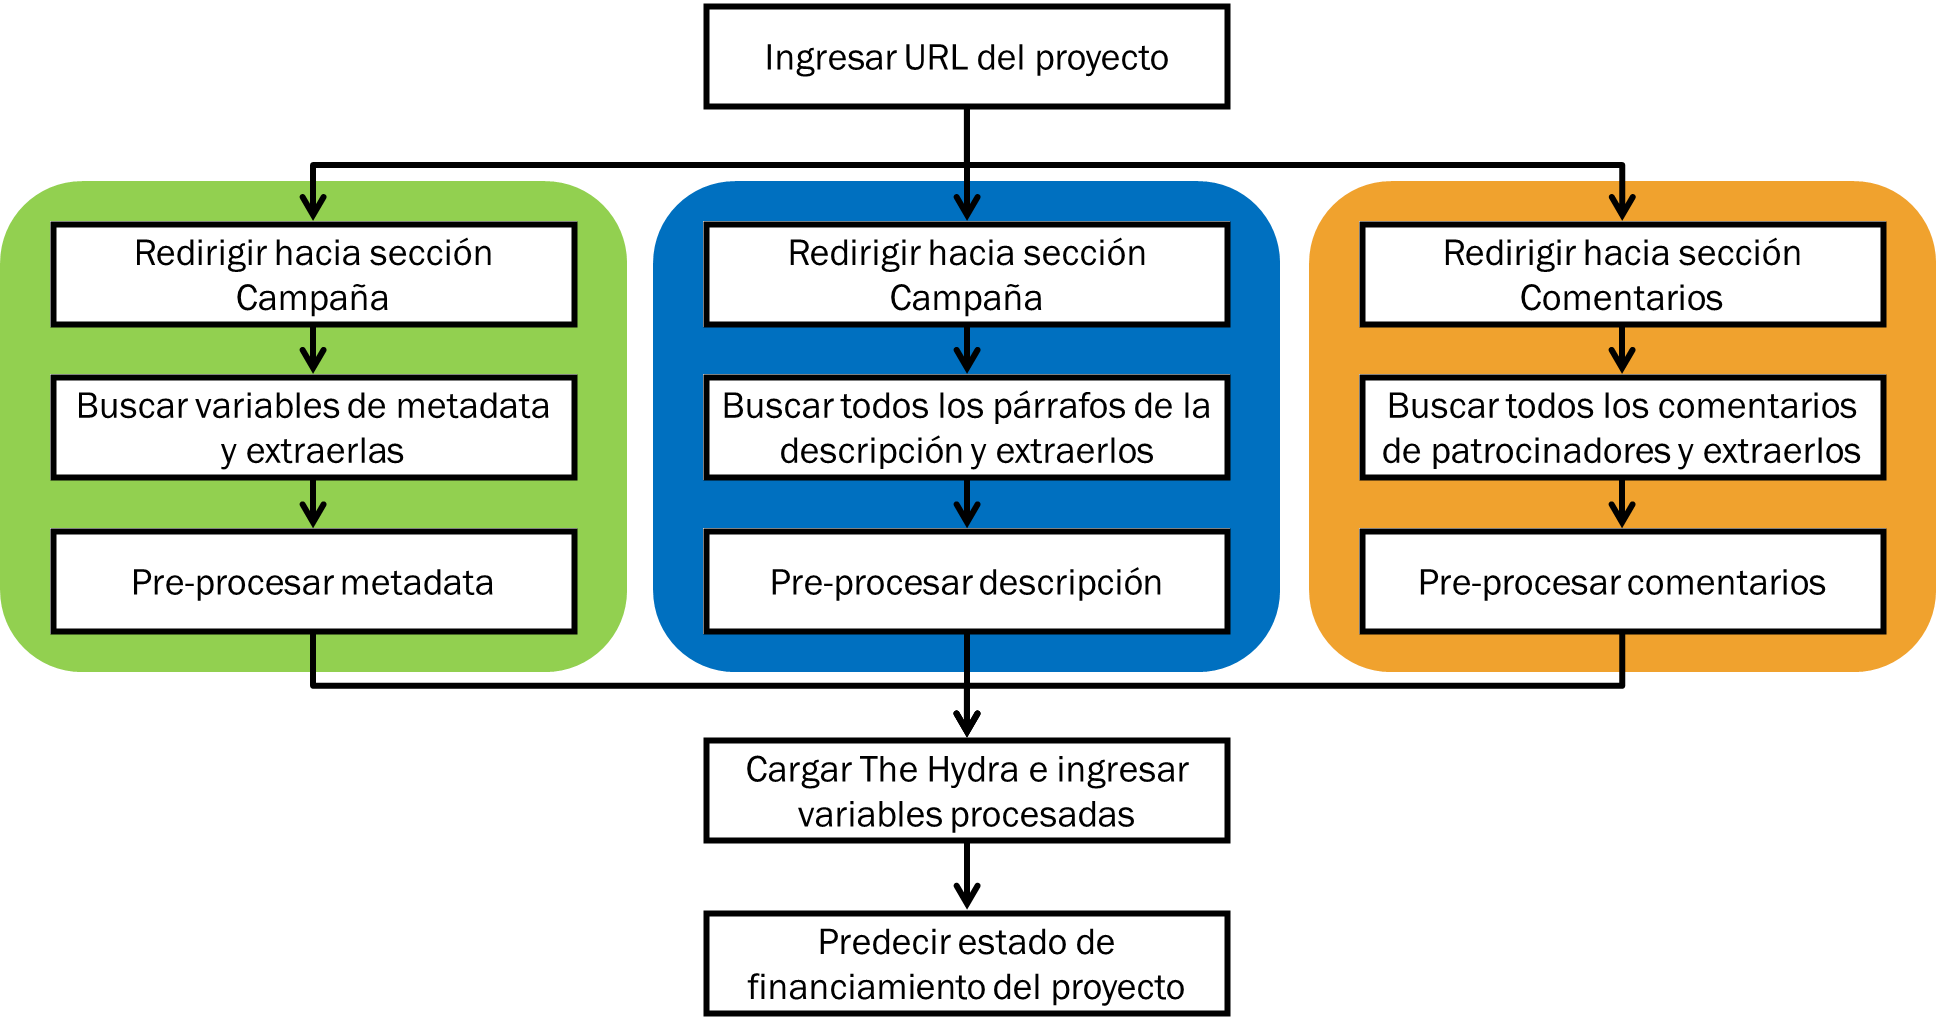
\includegraphics[width=0.95\textwidth]{5/figures/demo_flux.png}
		\caption[Proceso de operación del prototipo del sistema]{Proceso de operación del prototipo del sistema.\\
			Fuente: Elaboración propia.}
		\vspace{-0.75cm}
		\label{3:fig10}
	\end{center}
\end{figure}

\textbf{Entregable}: Arquitectura del prototipo del sistema integrado.

\vspace{0.25cm}
\textbf{Actividad 2: Ejecutar prototipo con proyectos tecnológicos vigentes}
\\
En esta actividad, se ejecutan las acciones de la arquitectura del prototipo mencionadas en la figura anterior. Comienza desde la captura de datos del proyecto consultado a través de su dirección web y culmina con la predicción de su estado de financiamiento.

\textbf{Entregable}: Predicción del proyecto consultado.

\vspace{0.5cm}
\subsection{Metodología para la medición de resultados}
Para evaluar la performance de un modelo, que representa la quinta fase de la metodología CRISP-DM, se utilizan diversas métricas como instrumentos de medición de desempeño a partir de los resultados arrojados en la Matriz de confusión. A continuación, se detalla su concepto y sus elementos.

\begin{itemize}
	\item \textbf{Matriz de confusión}: Es una tabla de NxN que resume el nivel de éxito de las predicciones de un modelo de clasificación; es decir, la correlación que existe entre la etiqueta y la clasificación del modelo. Un eje de una matriz de confusión es la etiqueta que el modelo predijo; el otro es la etiqueta real. N representa el número de clases. Es un problema de clasificación binaria, N=2 \parencite{gl_kohavi1998ml_glossary}. Su principal objetivo es describir el rendimiento de un modelo supervisado de Machine Learning en los datos de prueba, donde se desconocen los verdaderos valores. Se le llama “matriz de confusión” porque hace que sea fácil detectar dónde el sistema está confundiendo dos clases \parencite{gl_bigdata2019metricas}. Se representa en la Tabla \ref{2:table2}.
	
	\begin{table}[h!]
		\caption[Matriz de confusión]{Matriz de confusión.}
		\label{2:table2}
		\centering
		\small
		\begin{tabular}{llcc}
			\specialrule{.1em}{.05em}{.05em}
			&                                                            & \multicolumn{2}{c}{Valores Actuales}
			\\
			\cline{3-4} 
			& \multicolumn{1}{l}{}                                      & \multicolumn{1}{c}{Positivos (1)} & \multicolumn{1}{c}{Negativos (0)}
			\\
			\specialrule{.1em}{.05em}{.05em}
			\multicolumn{1}{c}{}                                             & \multicolumn{1}{c}{Positivos (1)} & \multicolumn{1}{c}{Verdaderos Positivos (VP)}             & \multicolumn{1}{c}{Falsos Positivos (FP)}                 \\ \cline{2-4} 
			\multicolumn{1}{c}{\multirow{-2}{*}{Valores Predichos}} & \multicolumn{1}{c}{Negativos (0)} & \multicolumn{1}{c}{Falsos Negativos (FN)}                 & \multicolumn{1}{c}{Verdaderos Negativos (VN)}
			\\
			\specialrule{.1em}{.05em}{.05em}
		\end{tabular}
		\par	%%Salto de linea
		\bigskip
		\begin{flushleft}	%%Alinear a la izquierda sin justificar
			\small Fuente: \cite{gl_izco2018bdc}
		\end{flushleft}
	\end{table}	
\end{itemize}

\begin{itemize}
	\item \textbf{Verdadero positivo} (TP o \textit{True Positive}): Es el ejemplo en el que el modelo predijo de manera correcta la clase positiva. Por ejemplo, el modelo infirió correctamente que un paciente con determinadas características descritas en las variables sufre de cáncer \parencite{gl_google2018machinelearning}.
	\item \textbf{Verdadero negativo} (TN o \textit{True Negative}): Es el ejemplo en el que el modelo predijo de manera correcta la clase negativa. Por ejemplo, el modelo infirió correctamente que una determinada especie animal de acuerdo a sus características no era un mamífero \parencite{gl_google2018machinelearning}.
	\item \textbf{Falso positivo} (FP, \textit{False Positive} o Error del Tipo I): Es el ejemplo en el que el modelo predijo de manera incorrecta la clase positiva. Por ejemplo, el modelo infirió que un paciente varón presentaba embarazo (clase positiva) cuando en realidad no era así \parencite{gl_google2018machinelearning}.
	\item \textbf{Falso negativo} (FN, \textit{False Negative} o Error del Tipo II): Es el ejemplo en el que el modelo predijo de manera incorrecta la clase negativa. Por ejemplo, el modelo infirió que un mensaje de correo electrónico en particular no era spam (clase negativa), pero ese mensaje en realidad sí era spam \parencite{gl_google2018machinelearning}. 
\end{itemize}

Explicado los conceptos anteriores, se derivan las siguientes métricas de clasificación usadas comúnmente, de las cuales serán usadas solo las 3 primeras tomando como referencia los papers de los antecentes:
\begin{itemize}
	\item \textbf{Exactitud} (\textit{accuracy}): Representa la fracción de predicciones que se realizaron correctamente sobre el total de ejemplos en un modelo de clasificación. Se determina mediante la siguiente fórmula \parencite{gl_kohavi1998ml_glossary}:
	
	%\begin{equcaption}[!ht]
	\begin{equation}\label{eq:accuracy}
	\phantomsection
	Exactitud=\frac{V.P.+V.N.}{V.P.+V.N.+F.P.+F.N.}
	\end{equation}
	\myequations{Fórmula para calcular la exactitud}
	%\caption[Fórmula para calcular la exactitud]{Fórmula para calcular la exactitud. Fuente: \cite{gl_kohavi1998ml_glossary}}
	%\end{equcaption}
	
	Esta métrica responde a la pregunta ¿Cuál es la proporción de predicciones que se realizaron correctamente? \parencite{gl_izco2018bdc}
	
	\item \textbf{Precisión} (\textit{precision}): Representa el número de elementos identificados correctamente como positivo de un total de elementos identificados como positivos \parencite{gl_bigdata2019metricas}. Se calcula mediante la siguiente fórmula:
	
	%\begin{equcaption}[!ht]
	\begin{equation}\label{eq:precision}
	\phantomsection
	Precisi\acute{o}n=\frac{V.P.}{V.P.+F.P.}
	\end{equation}
	\myequations{Fórmula para calcular la precisión}
	%\caption[Fórmula para calcular la precisión]{Fórmula para calcular la precisión. Fuente: \cite{gl_kohavi1998ml_glossary}}
	%\end{equcaption}
	
	Esta métrica responde a la pregunta ¿Qué proporción de predicciones positivas es correcta? \parencite{gl_izco2018bdc}
	
	\item \textbf{Área bajo la curva ROC} (\textit{AUC}): Considera todos los umbrales de clasificación posibles. Representa la probabilidad de que un clasificador tenga más seguridad de que un ejemplo resulte ser un verdadero positivo con respecto a que sea un falso positivo \parencite{gl_google2018machinelearning}. Para entender el concepto del área, se necesita entender qué es la curva ROC y para qué sirve en primer lugar.
	
	La curva ROC permite cuantificar la performance de distinción entre dos cosas del modelo como, por ejemplo, si un paciente tiene cáncer o no.
	
	Siguiendo el anterior ejemplo, se tiene un modelo que predice si un paciente sufre de cáncer o no, cuyo resultado es el siguiente (Figura \ref{3:fig11})
	
	\begin{figure}[htbp]
		\begin{center}
			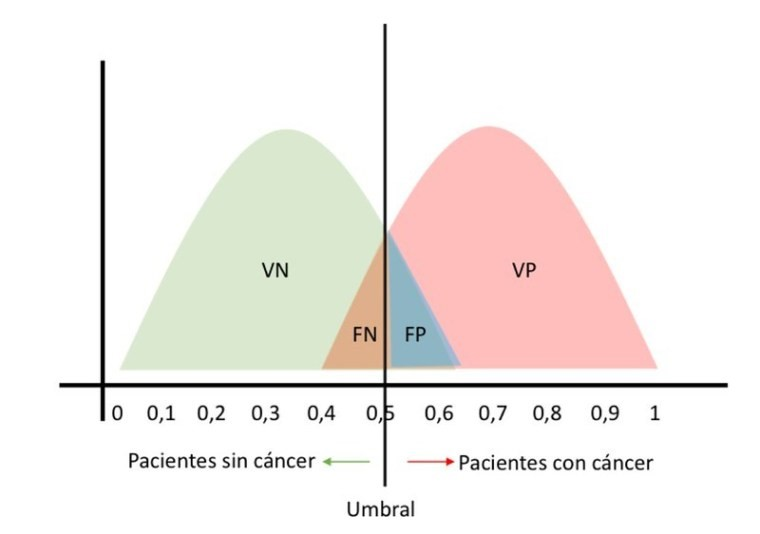
\includegraphics[width=0.55\textwidth]{3/figures/auc_example.jpg}
			\caption[Descripción de resultados de modelo descriptivo de ejemplo]{Descripción de resultados de modelo descriptivo de ejemplo.\\
				Fuente: \cite{gl_gonzalez2019auc}. \textit{Curvas ROC y Área bajo la curva (AUC)}.}
			\label{3:fig11}
		\end{center}
	\end{figure}
	
	En esta imagen, se puede observar que el área de borde verde (que contiene a los Falsos Positivos y el total de Negativos) representa a todos los pacientes que no tienen cáncer, mientras que el área de borde rojo (que contiene a los Falsos Negativos y el total de Positivos) representa a todos los pacientes que sí tienen cáncer. El umbral, que está establecido con valor 0.5, representa el punto de corte en el que el modelo clasificará a todos los pacientes por encima de ese valor como positivos, es decir, que sí tienen cáncer; mientras que aquellos por debajo del valor del umbral serán clasificados como negativos, es decir, que no tienen cáncer.
	
	Cuando el umbral se desplaza hacia la izquierda, es decir, cuando la sensibilidad aumenta, la especificidad disminuirá. Por el contrario, cuando el umbral se desplaza hacia la derecha, la sensibilidad disminuirá y la especificidad aumentará. Se concluye entonces que existe una relación inversa entre la sensibilidad y la especificidad. En la curva ROC se representa la sensitividad (1-especificidad) \parencite{gl_gonzalez2019auc}.
	
	Ahora bien, el área que se grafica bajo esta curva explicará qué tan bien funciona el modelo. Este tendrá un mejor desempeño si la curva se aleja de la diagonal principal como se observa en la Figura \ref{3:fig12} y se calcula con la siguiente fórmula:
	
	\begin{equation}\label{eq:auc}
	\phantomsection
	P( score(x^{+}) > score(x^{-}) )
	\end{equation}
	\myequations{Fórmula para calcular el área bajo la curva ROC}
	
	\begin{figure}[htbp]
		\begin{center}
			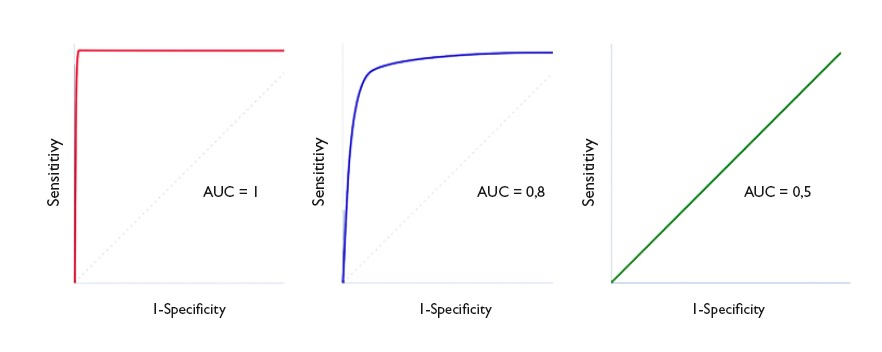
\includegraphics[width=1\textwidth]{3/figures/auc_curves.jpg}
			\caption[Comparación de tres resultados de la curva AUC en el modelo]{Comparación de tres resultados de la curva AUC en el modelo.\\
			Fuente: \cite{gl_molina2017pediatria_curvaroc}. \textit{Pruebas diagnósticas con resultados continuos o politómicos. Curvas ROC}. (p. 4)}
			\label{3:fig12}
		\end{center}
	\end{figure}
	
	Una interpretación básica del área bajo la curva ROC respecto del poder discriminante del modelo se muestra a continuación \parencite{bk_britos2006datamining}:
	\begin{itemize}
		\item Si el área bajo la curva ROC = 0.5, entonces el poder discriminante del modelo es nulo.
		\item Si el área bajo la curva 0.5 $<$ ROC $<$ 0.7, entonces el poder discriminante del modelo no es aceptable.
		\item Si el área bajo la curva 0.7 $\leq$ ROC $<$ 0.8, entonces el poder discriminante del modelo es aceptable.
		\item Si el área bajo la curva 0.8 $\leq$ ROC $<$ 0.9, entonces el poder discriminante del modelo es excelente.
		\item Si el área bajo la curva ROC $\geq$ 0.9, entonces el poder discriminante del modelo es excepcionalmente bueno.
	\end{itemize}
	\item \textbf{Sensibilidad} (\textit{recall}, \textit{sensitivity} o \textit{True Positive Rate}): Representa el número de elementos correctamente identificados como positivos del total de positivos verdaderos \parencite{gl_bigdata2019metricas}. Se calcula mediante la siguiente fórmula:
	
	%\begin{equcaption}[!ht]
	\begin{equation}\label{eq:recall}
	\phantomsection
	Sensibilidad=\frac{V.P.}{V.P.+F.N.}
	\end{equation}
	\myequations{Fórmula para calcular la sensibilidad}
	%\caption[Fórmula para calcular la sensibilidad]{Fórmula para calcular la sensibilidad. Fuente: \cite{gl_kohavi1998ml_glossary}}
	%\end{equcaption}
	
	\item \textbf{Puntaje F1} (\textit{F1-Score}): Representa la media armónica de la precisión y la sensibilidad. Normalmente, se usa cuando uno difiere mucho del otro y no es posible realizar una conclusión determinante ya que solo es posible predecir bien una clase \parencite{gl_bigdata2019metricas}. Se calcula mediante la siguiente fórmula:
	
	%\begin{equcaption}[!ht]
	\begin{equation}\label{eq:f1-score}
	\phantomsection
	Puntaje F1=\frac{2*Precisi\acute{o}n*Sensibilidad}{Precisi\acute{o}n+Sensibilidad}
	\end{equation}
	\myequations{Fórmula para calcular el puntaje F1}
	%\caption[Fórmula para calcular el puntaje F1]{Fórmula para calcular el puntaje F1. Fuente: \cite{gl_kohavi1998ml_glossary}}
	%\end{equcaption}
	
\end{itemize}

La elección de las anteriores métricas para evaluar cada modelo por modalidad y el modelo ensamblado propuesto se dio luego de realizar benchmarking sobre aquellas que fueron utizadas por los autores en los antecedentes de la investigación.

\begin{itemize}
	\item \textbf{Exactitud}: \cite{pr_chen2013kickpredict}, \cite{pr_chen2015predcrowd}, \cite{pr_beckwith2016predcrowd}, \cite{pr_yuan2016textanalytics}, \cite{pr_sawhney2016usingLT}, \cite{pr_kaur2017socmedcrowd}, \cite{pr_kamath2018suplearn}, \cite{pr_yu2018deeplearning}, \cite{pr_lee2018contentDL}, \cite{pr_cheng2019deeplearning}, \cite{pr_chen2019keywords_crowdfunding}, \cite{pr_shafqat2019topicpredictions}.
	\item \textbf{Precisión}: \cite{pr_beckwith2016predcrowd}, \cite{pr_yuan2016textanalytics}, \cite{pr_kaur2017socmedcrowd}, \cite{pr_cheng2019deeplearning}.
	\item \textbf{Sensibilidad}: \cite{pr_beckwith2016predcrowd}, \cite{pr_yuan2016textanalytics}, \cite{pr_kaur2017socmedcrowd}, \cite{pr_cheng2019deeplearning}, \cite{pr_chen2019keywords_crowdfunding}.
	\item \textbf{Especificidad}: \cite{pr_chen2019keywords_crowdfunding}.
	\item \textbf{Ratio de Falsa Alarma}: \cite{pr_kaur2017socmedcrowd}.
	\item \textbf{Media Geométrica (G-Mean)}: \cite{pr_chen2019keywords_crowdfunding}.
	\item \textbf{Puntaje F1}: \cite{pr_zhou2015projectdesc}, \cite{pr_beckwith2016predcrowd}, \cite{pr_yuan2016textanalytics}, \cite{pr_kaur2017socmedcrowd}, \cite{pr_cheng2019deeplearning}, \cite{pr_chen2019keywords_crowdfunding}.
	\item \textbf{Curva ROC}: \cite{pr_zhou2015projectdesc}, \cite{pr_beckwith2016predcrowd}.
	\item \textbf{Área bajo la Curva ROC (AUC)}: \cite{pr_beckwith2016predcrowd}, \cite{pr_li2016predcrowd}, \cite{pr_kaur2017socmedcrowd}, \cite{pr_yu2018deeplearning}, \cite{pr_cheng2019deeplearning}.
	\item \textbf{Área bajo la Curva Precisión-Sensibilidad (PRC)}: \cite{pr_kaur2017socmedcrowd}.
	\item \textbf{Error de Validación Cruzada}: \cite{pr_mitra2014phrases}.
	\item \textbf{Coeficiente de Correlación de Matthew (MCC)}: \cite{pr_kaur2017socmedcrowd}.
	\item \textbf{Divergencia de Kullback-Leibler (KL)}: \cite{pr_jin2019dayssuccess}.
	\item \textbf{Raíz del Error Cuadrático Medio (RMSE)}: \cite{pr_jin2019dayssuccess}.
	\item \textbf{Error Absoluto Medio (MAE)}: \cite{pr_jin2019dayssuccess}.
	\item \textbf{Índice de Concordancia (CI)}: \cite{pr_jin2019dayssuccess}.
\end{itemize}

\begin{landscape}
	\section{Cronograma de actividades y presupuesto}
	Se elaboró un cronograma de actividades de toda la investigación, mostrada en la Figura \ref{3:fig13}, contemplando desde el inicio de la misma a mediados del 2020 hasta la sustentación del trabajo estimado para finales de mayo del 2021.
	
	\begin{figure}[!ht]
		\begin{center}
			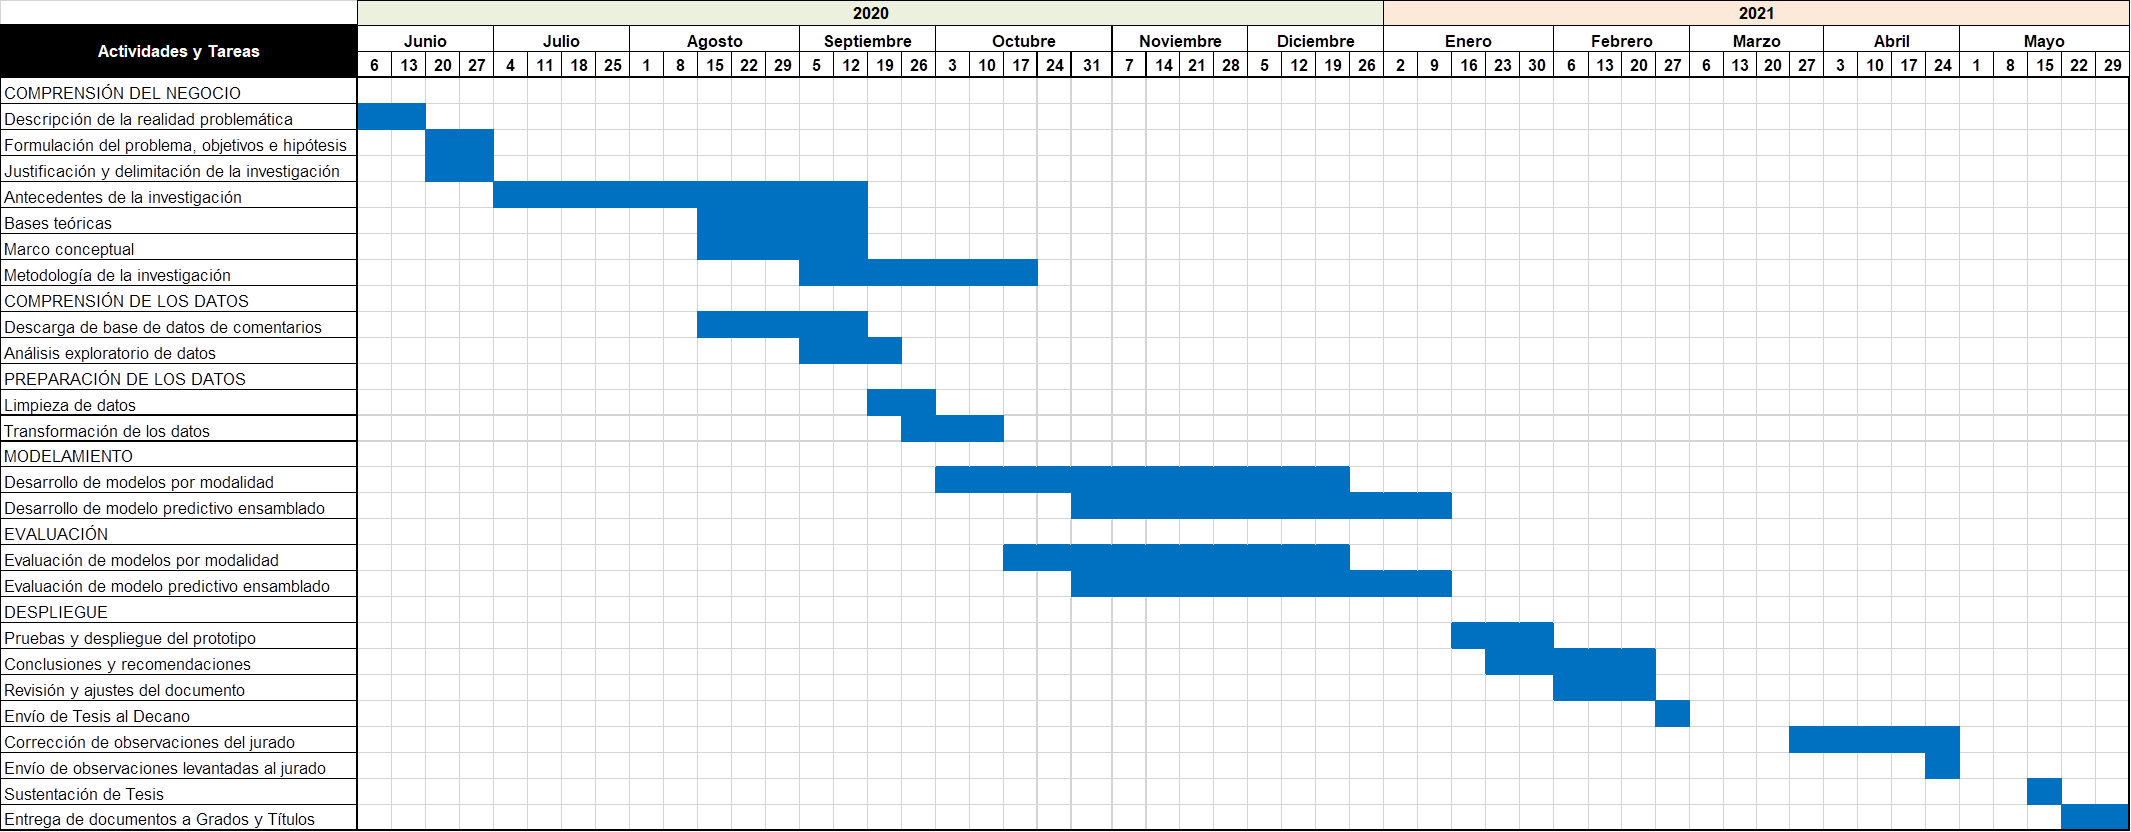
\includegraphics[width=1.55\textwidth]{3/figures/cronograma.png}
			\caption[Cronograma de actividades de la investigación]{Cronograma de actividades de la investigación.\\
				Fuente: Elaboración propia.}
			\label{3:fig13}
		\end{center}
	\end{figure}
	
\end{landscape}

Los costos personales del autor de la investigación se muestran en la Tabla \ref{3:table9}. Estos incluyen las herramientas adquiridas antes del inicio de la investigación como la laptop, así como pagos de servicios generales y del trámite de elaboración y sustentación pública de Tesis.

\begin{table}[h!]
	\caption[Presupuesto de los costos personales del autor]{Presupuesto de los costos personales del autor.}
	\label{3:table9}
	\centering
	\small
	\begin{tabular}{lcrr}
		\specialrule{.1em}{.05em}{.05em}
		\multicolumn{1}{c}{\centering{Item}} & \multicolumn{1}{c}{\centering{Tiempo usado (horas)}} & \multicolumn{1}{c}{\centering{Costo (soles)}} & \multicolumn{1}{c}{\centering{Subtotal}}
		\\
		\specialrule{.1em}{.05em}{.05em}
		\multicolumn{4}{l}{Recursos materiales}
		\\
		Laptop Lenovo ideapad 330 Core i7 8va Gen  &  & S/.4,500.00 & S/.4,500.00
		\\
		\hline
		\multicolumn{4}{l}{Pagos del trámite de elaboración y sustentación pública de Tesis}
		\\
		Derecho de inscripción de tema de investigación &  & S/.800.00 & S/.800.00
		\\
		Reserva del tema de tesis  &  & S/.2,700.00 & S/.2,700.00 \\
		Derecho de sustentación                                                          & & S/.1,500.00                                                                               & S/.1,500.00                                                                              \\
		\hline
		\multicolumn{4}{l}{Recursos humanos}
		\\
		Avance de tesis                                                                  & \multicolumn{1}{r}{900}                                                                    & Incalculable                                                                              & -                                                                                        \\
		\hline
		\multicolumn{4}{l}{Servicios generales}
		\\
		Internet + luz (7 meses)                                                         & \multicolumn{1}{r}{110}                                                                    & S/.80.00                                                                                  & S/.560.00                                                                              \\
		\specialrule{.1em}{.05em}{.05em}
		Total &  &  & \multicolumn{1}{l}{S/.10,060.00}
		\\
		\specialrule{.1em}{.05em}{.05em}
	\end{tabular}
	%\par	%%Salto de linea
	%\bigskip
	\begin{flushleft}	%%Alinear a la izquierda sin justificar
		\small Fuente: Elaboración propia.
	\end{flushleft}
\end{table}

Asimismo, también se contemplan los costos por uso de servicios en la nube como parte del proceso extracción de comentarios desde servidores en Google Cloud Platform (GCP) y desarrollo de modelos en Google Colab Pro en la Tabla \ref{3:table10}.

\begin{table}[h!]
	\caption[Presupuesto de los costos de las herramientas para el proyecto]{Presupuesto de los costos de las herramientas para el proyecto.}
	\label{3:table10}
	\centering
	\small
	\begin{tabular}{lcrcr}
		\specialrule{.1em}{.05em}{.05em}
		\multicolumn{1}{c}{\centering{Item}} & \multicolumn{1}{c}{\centering{Unidades}} & \multicolumn{1}{c}{\centering{Costo (dólares)}} & \multicolumn{1}{l}{\centering{Horas}} & \multicolumn{1}{c}{\centering{Subtotal}} \\
		\specialrule{.1em}{.05em}{.05em}
		\multicolumn{4}{l}{Google Cloud Platform} & -\$98.56
		\\
		Instancia VM Ubuntu (g1-small, 12GB RAM) & 1 & \$0.021 & 310 & \$6.51 \\
		Imagen de instancia Ubuntu & 8 & \$0.02 & 306 & \$48.96                                                                              \\
		Instancia VM de Windows Server 2019 (4GB RAM) & 1 & \$0.086 & 300 & \$25.80                                                                              \\
		Costo por instancias encendidas & 10 & & & \$3.41                                                                               \\
		Uso de instancias posteriormente eliminadas & & & & \$95.88                                                                              \\
		Pago mensual (luego de aceptar mejora de plan) & 4 & \$5.22 & & \$20.88                                                                              \\
		Crédito de \$300.00 por 12 meses & 1 & -\$300.00 & & -\$300.00                                                                            \\
		\hline
		\multicolumn{4}{l}{Google Colab Pro} & \$49.95
		\\
		Pago mensual (luego de aceptar mejora de plan) & 5 & \$9.99 & \multicolumn{1}{l}{} & \$49.95                                                                              \\
		\specialrule{.1em}{.05em}{.05em}
		Total a pagar &  &  &  & \$49.95
		\\
		\specialrule{.1em}{.05em}{.05em}
	\end{tabular}
	%\par	%%Salto de linea
	%\bigskip
	\begin{flushleft}	%%Alinear a la izquierda sin justificar
		\small Fuente: Elaboración propia.
	\end{flushleft}
\end{table}

Los montos por el uso de instancias creadas en GCP son descontados de los \$300.00 en crédito gratuito válidos por 12 meses \parencite{ot_googlecloud_freetrial}, recibidos inicialmente desde el 12 de agosto del 2020 para poder ser usados como versión de prueba. A partir del siguiente mes, se mejoró el plan para acceder a más servicios y comenzó a facturarse \$5.22 por mes.